\section{Trasformata Continua Di Fourier}
    \subsection{Segnali Aperiodici}
        Nel caso di segnali come $x_{(t)}=rect\left(\frac{t}{T}\right)$ non posso usare la $TSF$ posso peró scrivere:
        \[
            x_{(t)} = \lim_{T_0\rightarrow\infty} x_p(t) ,\ x_p(t) = \sum_{n = -\infty}^{\infty} x_{(t-nT_0)} 
        \]
        Passiamo da un analisi a frequenze discrete ad un analisi su tutto lo spettro delle frequenze
        \begin{figure}[H]
            \centering
            \subfloat[Spettro di Ampiezza TSF]{
                    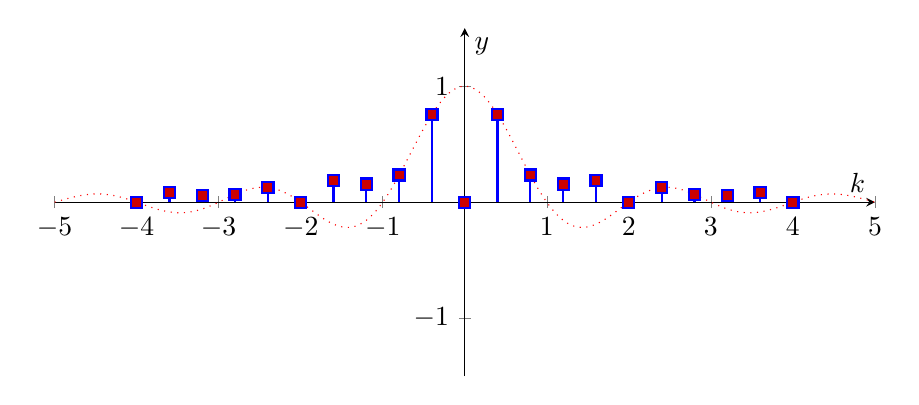
\begin{tikzpicture}
                        \begin{axis}[
                            domain=-5:5,
                            samples=200,
                            axis lines=middle,
                            xlabel=$k$,
                            ylabel=$y$,
                            ymin=-1.5,
                            ymax=1.5,
                            xtick={-5,-4,-3,-2,-1,0,1,2,3,4,5},
                            xticklabels={$-5$,$-4$,$-3$,$-2$,$-1$,$0$,$1$,$2$,$3$,$4$,$5$},
                            ytick={-1, 1},
                            yticklabels={$-1$, $1$},
                            width=12cm,
                            height=6cm
                        ]
                        \addplot [red,dotted, samples = 500] {sin(deg(x*pi))/(x*pi)};
                        \addplot+ [blue, thick, ycomb, samples at={-4,-3.6,-3.2,-2.8,-2.4,-2,-1.6,-1.2,-0.8,-0.4,0,0.4,0.8,1.2,1.6,2,2.4,2.8,3.2,3.6,4}] {abs(sin(deg(x*pi))/(x*pi))};
                        \end{axis}
                    \end{tikzpicture}
                }
                \hfill
                \subfloat[Spettro di Ampiezza TCF]{
                    \begin{tikzpicture}
                        \begin{axis}[
                            domain=-5:5,
                            samples=200,
                            axis lines=middle,
                            xlabel=$f$,
                            ylabel=$y$,
                            ymin=-1.5,
                            ymax=1.5,
                            xtick={-5,-4,-3,-2,-1,0,1,2,3,4,5},
                            xticklabels={$-5$,$-4$,$-3$,$-2$,$-1$,$0$,$1$,$2$,$3$,$4$,$5$},
                            ytick={-1, 1},
                            yticklabels={$-1$, $1$},
                            width=12cm,
                            height=6cm
                        ]
                        \addplot [red,dotted, samples = 300] {sin(deg(x*pi))/(x*pi)};
                        \addplot [blue, thick, samples = 300] {abs(sin(deg(x*pi))/(x*pi))};
                    \end{axis}
                    \end{tikzpicture}
                }
        \end{figure}

    \subsection{Equazioni di Analisi e Sintesi}
        \begin{figure}[H]
            \centering
            \includegraphics[width=12cm]{media/insiemi_tcf.png}
            \caption{Insiemi dei segnali per tcf}
            \label{fig:segnali aperiodici tcf}
        \end{figure}
        {\subsubsection{Equazione di Analisi}
            \[X_{(f)} = \int_{-\infty}^{\infty} x_{(t)} e^{-j2\pi ft} dt\hspace{0.3cm} Equazione\ di\ analisi \]
            
        \subsubsection{Equazione di Sintesi}
            \[x_{(t)} = \int_{-\infty}^{\infty} X_{(f)} e^{j2\pi ft} df\hspace{0.3cm} Equazione\ di\ sintesi \]
        }
        La $TCF$ gode della biunivocitá
        \begin{align}
            x_{(t)} \overunderset{TCF}{ATCF}{\leftrightharpoons}  X_{(f)}\nonumber \hspace{0.3cm} X_{(f)} \in \mathbb{C}
        \end{align}
        Essendo $X_k$ un numero complesso puó essere rappresentato in forma polare: 
        \[
            X_{(f)} = |X_{(f)}|e^{\angle X_{(f)}}  
        \]
        Si possono rappresentare il modulo (Ampiezza) e la fase tramite grafici che prendono il nome di spettri:
        \begin{figure}[H]
            \centering
            \subfloat[Spettro di Ampiezza]{
                    \begin{tikzpicture}
                        \begin{axis}[
                            domain=-5:5,
                            samples=200,
                            axis lines=middle,
                            xlabel=$f$,
                            ylabel=$y$,
                            ymin=-1.5,
                            ymax=1.5,
                            xtick={-5,-4,-3,-2,-1,0,1,2,3,4,5},
                            xticklabels={$-5$,$-4$,$-3$,$-2$,$-1$,$0$,$1$,$2$,$3$,$4$,$5$},
                            ytick={-1, 1},
                            yticklabels={$-1$, $1$},
                            width=12cm,
                            height=6cm
                        ]
                        \addplot [red,dotted, samples = 300] {sin(deg(x*pi))/(x*pi)};
                        \addplot [blue, thick, samples = 300] {abs(sin(deg(x*pi))/(x*pi))};
                    \end{axis}
                    \end{tikzpicture}
                }
            \hfill
            \subfloat[Spettro di Fase]{
                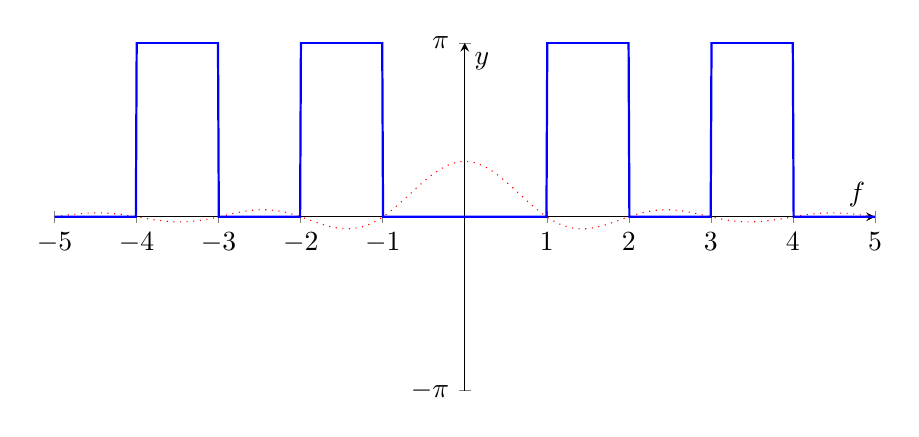
\begin{tikzpicture}
                    \begin{axis}[
                        domain=-5:5,
                        samples=200,
                        axis lines=middle,
                        xlabel=$f$,
                        ylabel=$y$,
                        ymin=-pi,
                        ymax=pi,
                        xtick={-5,-4,-3,-2,-1,0,1,2,3,4,5},
                        xticklabels={$-5$,$-4$,$-3$,$-2$,$-1$,$0$,$1$,$2$,$3$,$4$,$5$},
                        ytick={-pi, pi},
                        yticklabels={$-\pi$, $\pi$},
                        width=12cm,
                        height=6cm
                    ]
                    \addplot [red,dotted, samples = 300] {sin(deg(x*pi))/(x*pi)};
                    \addplot [blue, thick, samples = 1000] {rad(atan2(0,sin(deg(x*pi))/(x*pi)))};
                    \end{axis}
                \end{tikzpicture}
            }
            \caption{Spettro del segnale TCF}
        \end{figure}
        lo spettro di Ampiezza gode della \textbf{simmetria pari} rispetto alle ascisse quindi é \textbf{sempre positivo e continuo}, mentre lo spettro di fase della \textbf{simmetria dispari}, 
        questa propietá é chiamata \textbf{Simmetria Hermitiana}

        \subsubsection{TCF di una $Arect\left(\frac{t}{T}\right)$}
            $x_{(t)} = A\hspace{0.1cm}rect\left(\frac{t}{T}\right)$
            \begin{figure}[H]
                \centering
                \begin{tikzpicture}
                    \begin{axis}[
                        xlabel=$x$,
                        ylabel=$y$,
                        xmin=-5,
                        xmax=5,
                        ymin=-0.5,
                        ymax=4,
                        ytick = {1.5},
                        xtick={-1.5, 0, 1.5},
                        xticklabels={$-\frac{T}{2}$, $0$, $\frac{T}{2}$},
                        yticklabels = {$A$},
                        yticklabel style = {yshift=5pt,xshift=4pt}, 
                        axis lines=middle,
                        thick,
                        domain=-5:5,
                        samples=100,
                        width=8cm,
                        height=4cm
                    ]
                    \addplot [const plot,red, thick] coordinates{(-1.5,1.5)(1.5,1.5)};
                    \addplot [const plot,red, thick] coordinates{(-1.5,0)(-1.5,1.5)};
                    \addplot [const plot,red, thick] coordinates{(1.5,0)(1.5,1.5)};
                    \addplot [const plot,red, thick] coordinates{(5,0)(1.5,0)};
                    \addplot [const plot,red, thick] coordinates{(-5,0)(-1.5,0)};
                    \end{axis}
                  \end{tikzpicture}
                \caption{$A\hspace{0.1cm}rect\left(\frac{t}{T}\right)$}
                \label{fig:grafo rect nella tcf}
            \end{figure}
            $X_{(f)} = ? :$
            \begin{align}
                X_{(f)} & = \int_{-\infty}^{\infty} x_{(t)} e^{-j2\pi ft} dt \nonumber = \int_{-\frac{T}{2}}^{\frac{T}{2}} A\hspace{0.1cm}rect\left(\frac{t}{T}\right) e^{-j2\pi ft} dt \nonumber\\ 
                        & = A \int_{-\frac{T}{2}}^{\frac{T}{2}} e^{-j2\pi ft} dt = -\frac{A}{j2\pi f} \eval{e^{-j2\pi ft}}_{-\frac{T}{2}}^{\frac{T}{2}} =-\frac{A}{j2\pi f} \left(e^{-j\pi fT} - e^{j\pi fT}\right) \nonumber\\
                        & = \frac{A\color{purple}{T}}{\pi f} \left(\frac{e^{j\pi fT} - e^{-j\pi fT}}{2j}\right) = \frac{A{\color{purple}T}\sin(\pi fT)}{\pi f\color{purple}{T}} = AT sinc(fT) =  X_{(f)} \nonumber 
            \end{align}
            \[
                A\hspace{0.1cm}rect\left(\frac{t}{T}\right) \overunderset{TCF}{ATCF}{\leftrightharpoons} AT sinc(fT)
            \]
            La sinc si annulla in $\frac{k}{T},\ k\in \mathbb{Z}$. Notiamo anche come la funzione di partenza sia reale e pari la TCF rispetti \ref{Parita}(si?):
            \begin{figure}[H]
                \centering

            \subfloat[Spettro di Ampiezza]{
                \begin{tikzpicture}
                    \begin{axis}[
                        domain=-5:5,
                        samples=200,
                        axis lines=middle,
                        xlabel=$f$,
                        ylabel=$y$,
                        ymin=-1.5,
                        ymax=1.5,
                        xtick={-5,-4,-3,-2,-1,0,1,2,3,4,5},
                        xticklabels={$-\frac{5}{T}$,$-\frac{4}{T}$,$-\frac{3}{T}$,$-\frac{2}{T}$,$-\frac{1}{T}$,$0$,$\frac{1}{T}$,$\frac{2}{T}$,$\frac{3}{T}$,$\frac{4}{T}$,$\frac{5}{T}$},
                        ytick={-1, 1},
                        yticklabels={$-1$, $1$},
                        width=12cm,
                        height=6cm
                    ]
                    \addplot [red,dotted, samples = 300] {sin(deg(x*pi))/(x*pi)};
                    \addplot [blue, thick, samples = 300] {abs(sin(deg(x*pi))/(x*pi))};
                \end{axis}
                \end{tikzpicture}
                }
            \hfill
            \subfloat[Spettro di Fase]{
                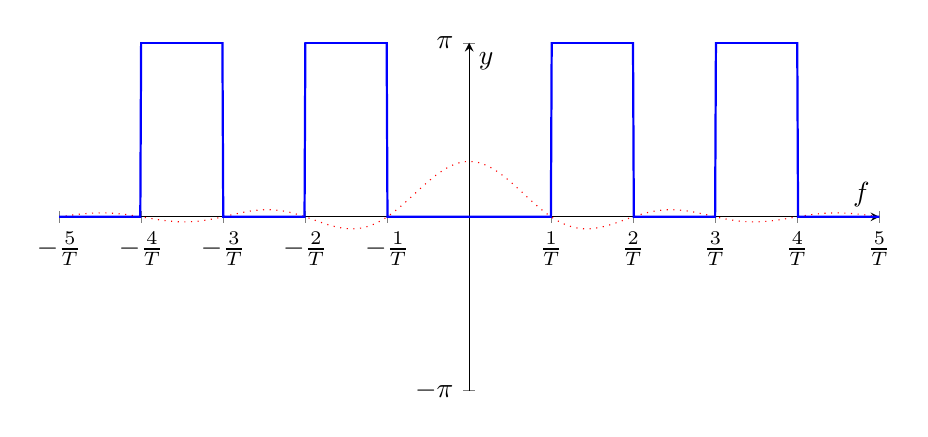
\begin{tikzpicture}
                    \begin{axis}[
                        domain=-5:5,
                        samples=200,
                        axis lines=middle,
                        xlabel=$f$,
                        ylabel=$y$,
                        ymin=-pi,
                        ymax=pi,
                        xtick={-5,-4,-3,-2,-1,0,1,2,3,4,5},
                        xticklabels={$-\frac{5}{T}$,$-\frac{4}{T}$,$-\frac{3}{T}$,$-\frac{2}{T}$,$-\frac{1}{T}$,$0$,$\frac{1}{T}$,$\frac{2}{T}$,$\frac{3}{T}$,$\frac{4}{T}$,$\frac{5}{T}$},
                        ytick={-pi, pi},
                        yticklabels={$-\pi$, $\pi$},
                        width=12cm,
                        height=6cm
                    ]
                    \addplot [red,dotted, samples = 300] {sin(deg(x*pi))/(x*pi)};
                    \addplot [blue, thick, samples = 1000] {rad(atan2(0,sin(deg(x*pi))/(x*pi)))};
                    \end{axis}
                \end{tikzpicture}
            }
            \end{figure}

    \subsection{Propietá}
        Come per la TSF vale che al variare del periodo della funzione $T$:
            \begin{itemize}
                \item Se $T\uparrow$ aumenta $ \rightarrow f\downarrow$ diminuisce e si stringe lo spettro  
                \item Se $T\downarrow$ diminuisce $ \rightarrow f\uparrow$ aumenta e si allarga lo spettro  
            \end{itemize}
        Inoltre come si puó evincere dal successivo Teorema della Dualitá \ref{Dualita}:
            \begin{itemize}
                \item Una funzione limitata (finita) nel tempo ha uno spettro nella frequenza illimitato $\rightarrow$ sono i segnali fisici   
                \item Una funzione illimitata nel tempo ha uno spettro nella frequenza limitato (finito)
            \end{itemize}

        \subsubsection{Simmetria hermitiana}\label{Simmetria Hermitiana}
            \begin{align}
                Ip&: x_{(t)}\ reale \nonumber \\
                Th&: X_{(f)}\ hermitiana \nonumber \\ 
                X_{(-f)} &= X_{(f)}^{*} \rightarrow
                    \begin{cases}
                        |X_{(f)}| = |X_{(-f)}| \hspace{0.3cm} & Simmetria\ Pari \\
                        \angle X_{(-f)} = -\angle X_{(f)}\hspace{0.3cm} & Simmetria\ Dispari
                    \end{cases} \nonumber
            \end{align}

        \subsubsection{Paritá}\label{Parita}
            \begin{align}
                Ip&: x_{(t)}\ reale\ e\ pari  \nonumber \\
                Th&: X_{(f)}\ reale\ e\ pari \nonumber  
            \end{align}

        \subsubsection{Disparitá}\label{Disparita}
            \begin{align}
                Ip&: x_{(t)}\ reale\ e\ dispari  \nonumber \\
                Th&: X_{(f)}\ immaginaria\ e\ dispari \nonumber 
            \end{align}

    \subsection{Teoremi relativi alla TCF}
        \subsubsection{Linearitá}\label{Linearita}
            $Ip: x_{(t)} = \alpha x_{1(t)} + \beta x_{2(t)}$\\        
            $Th: X_{(f)} = \alpha X_{1(f)} + \beta X_{2(f)}$\\ 
            Dimostrazione:
            \begin{align}
                X_{(f)} & = \int_{-\infty}^{\infty} (\alpha x_{1(t)} + \beta x_{2(t)}) e^{-j2\pi ft} dt \nonumber \\
                        & = \alpha \int_{-\infty}^{\infty} x_{1(t)} e^{-j2\pi ft} dt + \beta \int_{-\infty}^{\infty}  x_{2(t)} e^{-j2\pi ft} dt  \nonumber \\
                        & = \alpha X_{1(f)} + \beta X_{2(f)} \nonumber
            \end{align}

            Esempio:
                {   
                    \begin{align}
                        x_{(t)} &= A rect\left(\frac{t}{2T}\right) + Brect\left(\frac{t}{T}\right)\nonumber \\   
                        X_{(f)} &= A X_{1(f)} + B X_{2(f)} = 2AT sinc(2Tf) + BT sinc(Tf) \nonumber \\
                        X_{1(f)} &= 
                        \begin{cases}
                            X_{1(f)} = A rect\left(\frac{t}{T^\prime}\right) \overset{TCF}{\leftrightharpoons} T^\prime sinc(T^\prime f) \Rightarrow X_{1(f)} =2Tsinc(2Tf) \\
                            T^\prime = 2T
                        \end{cases} \nonumber
                    \end{align}
                    \begin{figure}[H]
                        \centering
                        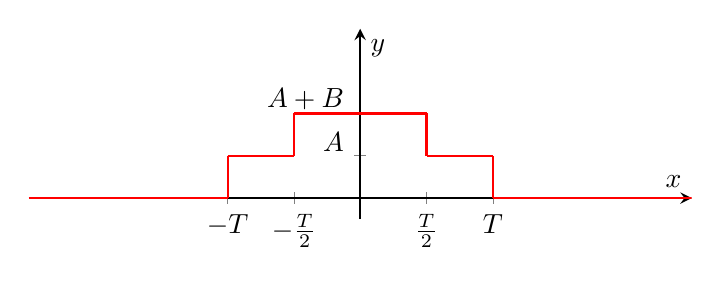
\begin{tikzpicture}
                            \begin{axis}[
                                xlabel=$x$,
                                ylabel=$y$,
                                xmin=-5,
                                xmax=5,
                                ymin=-0.5,
                                ymax=4,
                                ytick = {1,2},
                                yticklabels = {$A$,$A+B$},
                                xtick={-2,-1, 0, 1,2},
                                xticklabels={$-T$,$-\frac{T}{2}$, $0$, $\frac{T}{2}$,$T$},
                                yticklabel style = {yshift=5pt}, 
                                axis lines=middle,
                                thick,
                                domain=-5:5,
                                samples=100,
                                width=10cm,
                                height=4cm
                            ]
                            
                            \addplot [const plot,red, thick] coordinates{(-2,1)(-1,1)};
                            \addplot [const plot,red, thick] coordinates{(2,1)(1,1)};

                            \addplot [const plot,red, thick] coordinates{(1,1)(1,2)};
                            \addplot [const plot,red, thick] coordinates{(-1,1)(-1,2)};
                            \addplot [const plot,red, thick] coordinates{(-1,2)(1,2)};
                            
                            \addplot [const plot,red, thick] coordinates{(-2,0)(-2,1)};
                            \addplot [const plot,red, thick] coordinates{(2,0)(2,1)};


                            \addplot [const plot,red, thick] coordinates{(5,0)(2,0)};
                            \addplot [const plot,red, thick] coordinates{(-5,0)(-2,0)};
                            \end{axis}
                          \end{tikzpicture}
                        \caption{Segnale rettangolo}
                        \label{fig:es linearita}
                    \end{figure}                    
                }
                

        \subsubsection{Dualitá}\label{Dualita}
            $Ip: x_{(t)} \overunderset{TCF}{ATCF}{\leftrightharpoons} X_{(f)}$\\        
            $Th: X_{(t)} \overunderset{TCF}{ATCF}{\leftrightharpoons} x_{(-f)}$ 
            Dimostrazione:
            \begin{align}
                X_{(f)} & = \int_{-\infty}^{\infty} x_{(t)} e^{-j2\pi ft} dt = Sost. \begin{cases}
                    t \rightarrow f\\
                    f \rightarrow t
                \end{cases} \Rightarrow  X_{(t)} = \int_{-\infty}^{\infty} x_{(f)} e^{-j2\pi tf} df \nonumber \\
                        & =Sost.\ (f^\prime = -f) \Rightarrow  X_{(t)} = \int_{-\infty}^{\infty} x_{(-f^\prime)} e^{-j2\pi t(-f^\prime)} df^\prime\nonumber \\
                        & =\int_{-\infty}^{\infty} x_{(-f^\prime)} e^{j2\pi tf^\prime} df^\prime= ACTF[x_{(-f)}] = c.v.d.  \nonumber
            \end{align}
            Esempio:\\
                {
                    $x_{(t)}=Asinc(Bt) \Rightarrow X_{(f)} = \int_{-\infty}^{\infty}A sinc(Bt)e^{-j2\pi ft}dt$ \\
                    Applico la dualitá:
                    \begin{gather}
                        A rect\left(\frac{t}{T}\right) \rightleftarrows ATsinc(Tf) \nonumber \\
                        ATsinc(Tt) \rightleftarrows A rect\left(\frac{-f}{T}\right) \nonumber
                    \end{gather}
                    Se voglio una durata generica:
                    \begin{gather}
                        Sostituisco\ B=T \nonumber \\
                        ABsinc(Bt) \rightleftarrows A rect\left(\frac{f}{B}\right) \nonumber  \\
                        \Downarrow \nonumber \\
                        Asinc(Bt) \rightleftarrows \frac{A}{B}rect\left(\frac{f}{B}\right) \nonumber
                    \end{gather}
                }

        \subsubsection{Ritardo}\label{Ritardo}
            $Ip: x_{(t)} \overunderset{TCF}{ATCF}{\leftrightharpoons} X_{(f)},\ y_{(t)} = x_{(t-to)}$\\        
            $Th: Y_{(f)} \overunderset{TCF}{ATCF}{\leftrightharpoons} y_{(t)} = X_{(f)}e^{-j2\pi ft_0}$\\ 
            Dimostrazione:
            \begin{align}
                Y_{(f)} & = \int_{-\infty}^{\infty} y_{(t)} e^{-j2\pi ft} dt = \int_{-\infty}^{\infty} x_{(t-t_0)} e^{-j2\pi tf} dt \nonumber \\
                        & =Sost.\ (t^\prime = t-t_0) \Rightarrow  Y_{(f)} = \int_{-\infty}^{\infty} x_{(t^\prime)} e^{-j2\pi f(t^\prime+t_0)} dt^\prime \nonumber \\
                        & =\int_{-\infty}^{\infty} x_{(t^\prime)} e^{-j2\pi ft^\prime}e^{-j2\pi ft_0} dt^\prime= X_{(f)}e^{-j2\pi ft_0}\ c.v.d.  \nonumber
            \end{align}
            {\em Osservazione:}
                \begin{itemize}
                    \item Un ritardo nel tempo introduce una componente solo di fase che cresce lienarmente con la frequenza
                    \item Un esponenziale nel tempo introduce un ritardo nel dominio della frequenza $x_{(t)}e^{-j2\pi f_0t} \rightarrowtail X_{(f-f_0)}$, vedi \ref{Modulazione con Esponenziale Complesso}
                \end{itemize}
            Esempio:\\
                {
                    $x_{0(t)} = A rect\left(\frac{t}{T}\right) \rightarrow x_{(t)}=x_{0(t-t_0)}\hspace{0.3cm} t_0 = \frac{T}{2}$
                    \begin{figure}[H]
                        \centering
                        \begin{tikzpicture}
                            \begin{axis}[
                                xlabel=$t$,
                                ylabel=$y$,
                                xmin=-5,
                                xmax=5,
                                ymin=-0.5,
                                ymax=4,
                                ytick = {1.5},
                                yticklabels = {$A$},
                                yticklabel style = {yshift=8pt,xshift=4pt}, 
                                xtick={-1,0,1,2},
                                xticklabels={$-\frac{T}{2}$,$0$,$\frac{T}{2}$,$T$},
                                axis lines=middle,
                                thick,
                                domain=-5:5,
                                samples=100,
                                width=10cm,
                                height=5cm
                            ]
                            
                            \addplot [const plot, blue] coordinates{(-1,1.5)(1,1.5)};
                            \addplot [const plot, blue] coordinates{(-1,0)(-1,1.5)};
                            \addplot [const plot, blue] coordinates{(1,0)(1,1.5)};
                            
                            \addplot [const plot, purple] coordinates{(0,1.5)(2,1.5)};
                            \addplot [const plot, purple] coordinates{(0,0)(0,1.5)};
                            \addplot [const plot, purple] coordinates{(2,0)(2,1.5)};
                            
                            \end{axis}
                        \end{tikzpicture}
                        \caption{{\color{blue}$x_{0(t)}$}, {\color{purple}$x_{(t)}$}}
                        \label{fig:ritardo rect}
                    \end{figure}
                    \[
                        X_{(f)} = X_{0(f)}e^{-j2\pi f\frac{T}{2}} = AT sinc(Tf) e^{-j\pi fT}    
                    \]

                    \begin{figure}[H]
                        \centering
                        \subfloat[Ampiezza con ritardo]{
                            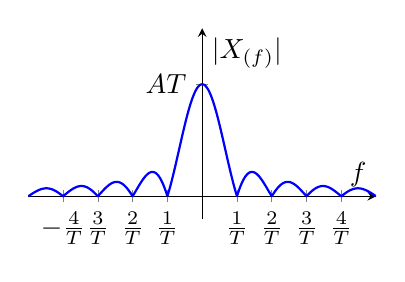
\begin{tikzpicture}
                                \begin{axis}[
                                    domain=-5:5,
                                    samples=200,
                                    axis lines=middle,
                                    xlabel=$f$,
                                    ylabel=$|X_{(f)}|$,
                                    ytick = {1},
                                    yticklabels = {$AT$},
                                    xtick = {-4,-3,-2,-1,0,1,2,3,4},
                                    xticklabels = {$-\frac{4}{T}$,$\frac{3}{T}$,$\frac{2}{T}$,$\frac{1}{T}$,$0$,$\frac{1}{T}$,$\frac{2}{T}$,$\frac{3}{T}$,$\frac{4}{T}$},
                                    ymin=-0.2,
                                    ymax=1.5,
                                    width=6cm,
                                    height=4cm
                                ]
                                \addplot [blue, thick, samples = 500] {abs(sin(deg(x*pi))/(x*pi))};
                                \end{axis}
                            \end{tikzpicture}
                            \label{fig:Ampiezza}
                        }
                        \hfill
                        \subfloat[Fase con ritardo]{
                                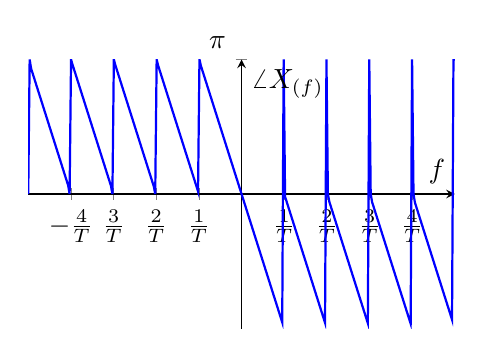
\begin{tikzpicture}
                                    \begin{axis}[
                                        domain=-5:5,
                                        samples=200,
                                        axis lines=middle,
                                        xlabel=$f$,
                                        ylabel=$\angle X_{(f)}$,
                                        ymin=-pi,
                                        ymax=pi,
                                        xtick = {-4,-3,-2,-1,0,1,2,3,4},
                                        xticklabels = {$-\frac{4}{T}$,$\frac{3}{T}$,$\frac{2}{T}$,$\frac{1}{T}$,$0$,$\frac{1}{T}$,$\frac{2}{T}$,$\frac{3}{T}$,$\frac{4}{T}$},
                                        ytick={pi},
                                        yticklabel style = {yshift=6pt}, 
                                        yticklabels={$\pi$},
                                        width=7cm,
                                        height=5cm
                                    ]
                                    \addplot [blue, thick, samples = 300] {rad(atan2((-((sin(deg(pi*x)))^2)/(pi*x)),((cos(deg(pi*x))*sin(deg(pi*x)))/(pi*x))))};
                                    \end{axis}
                                \end{tikzpicture}
                            \label{fig:fase}
                        }
                        \caption{Spettro della $rect$ con ritardo}
                    \end{figure}
                    Il \LaTeX{} sbaglia e aggiunge le spike nelle $f$ positive, il grafico é dispari con andamento come per le $f$ negative.
                }

        \subsubsection{Derivazione}\label{Derivazione}
            $Ip:\begin{cases}
                x_{(t)}\overunderset{TCF}{ATCF}{\leftrightharpoons} X_{(f)}\\
                y_{(t)}= \derivative{}{t} x_{(t)}        
            \end{cases}$\\
            $Th: Y_{(f)} = j2\pi f X_{(f)} $ \\
            Dimostrazione:\\
            \begin{align}
                y_{(t)} &= \derivative{}{t} x_{(t)} = \derivative{}{t} ACTF[x_{(t)}] =\derivative{}{t} \int_{-\infty}^{\infty} X_{(f)}e^{j2\pi ft} df = \nonumber\\
                        &= \int_{-\infty}^{\infty} X_{(f)}\derivative{}{t}e^{j2\pi ft} df = \int_{-\infty}^{\infty} X_{(f)}j2\pi fe^{j2\pi ft} df \nonumber
            \end{align}
            Posso Scrivere $y_{(t)}$ come $ACTF[y_{(t)}] = \int_{-\infty}^{\infty} Y_{(f)}e^{j2\pi ft} df $, se quindi $Y_{(f)} = j2\pi f X_{(f)}$ l'ugaglianza é valida:
            \[
                y_{(t)} =\int_{-\infty}^{\infty} Y_{(f)}e^{j2\pi ft} df
            \]
            L'operazione di derivata nel dominio della frequenza si traduce in una semplice operazione algebrica, nel tempo avrei dovuto calcolare il 
            rapporto incrementale. Per derivare un segnale posso quindi:
            \begin{gather}
                x_{(t)} \rightarrow TCF \rightarrow j2\pi fX_{(f)} \rightarrow ACTF \rightarrow y_{(t)}\nonumber
            \end{gather}
            
        \subsubsection{Integrazione}\label{Integrazione}
            $Ip:\begin{cases}
                x_{(t)} \overunderset{TCF}{ATCF}{\leftrightharpoons} X_{(f)}\ (1)\\
                y_{(t)} = \int_{-\infty}^{t} x_{(\alpha)} d\alpha\ (2) \\
                \int_{-\infty}^{\infty} x_{(t)} dt\ oppure\ \eval*{X_{(f)}}_{f=0} = 0 \ oppure\ y{(+\infty)} = 0\ (3) \\
            \end{cases}$\\
            $Th: Y_{(f)} =\frac{X_{(f)}}{j2\pi f}$ \\
            Dimostrazione:\\
            \begin{gather}
                y_{(t)} = \int_{-\infty}^{t} x_{(\alpha)} d\alpha \Rightarrow {\color{purple}\derivative{}{t}} x_{(t)} = {\color{purple}\derivative{}{t}} y_{(t)} \overset{Th. \ref{Derivazione}}{\Rightarrow}  X_{(f)} = j2\pi f Y_{(f)} \nonumber\\
                         Y_{(f)} =\frac{X_{(f)}}{j2\pi f}\nonumber
            \end{gather}

            L'ipotesi 3 é conseguenza della divisione per $f$ e che devo mantenere l'uguaglianza $X_{(f)} = j2\pi f Y_{(f)}$, si nota come nella dimostrazione usando il Th della Derivazione (\ref{Derivazione})
            quando $f=0$ la funzione nella frequenza deve essere $0,\ X_{(f)} = j2\pi f Y_{(f)} = 0$ 
        
        Esempio: $TCF$ di una piramide\\
        {
            \[
                x_{(t)} = A\left(1-\left(\frac{|t|}{T}\right)\right)rect \left(\frac{t}{2T}\right) \hspace{0.3cm} X_{(f)} = TCF[x_{(t)}] = ?
            \]
            \begin{figure}[H]
                \centering
                \begin{tikzpicture}
                    \begin{axis}[
                        xlabel=$t$,
                        ylabel=$x_{(t)}$,
                        xmin=-5,
                        xmax=5,
                        ymin=-0.5,
                        ymax=3,
                        ytick = {2},
                        yticklabels = {$A$},
                        xtick={-2,0,2},
                        xticklabels={$-T$,$0$,$T$},
                        axis lines=middle,
                        thick,
                        domain=-5:5,
                        samples=100,
                        width=10cm,
                        height=5cm
                    ]
                    
                    \addplot [sharp plot, blue] coordinates{(-2,0)(0,2)};
                    \addplot [sharp plot, blue] coordinates{(2,0)(0,2)};
                    \addplot [sharp plot, blue] coordinates{(2,0)(5,0)};
                    \addplot [sharp plot, blue] coordinates{(-2,0)(-5,0)};

                    \end{axis}
                \end{tikzpicture}
                \caption{Funzione priamide}
                \label{fig:funzione piramide}
            \end{figure}
            $TCF[x_{(t)}]:$
            \begin{itemize}
                \item {
                    Utilizzando la classica $TCF$:\\     
                        \[X_{(f)} = \int_{-\infty}^{\infty} A\left(1-\left(\frac{|t|}{T}\right)\right)rect \left(\frac{t}{2T}\right) dt\]
                }
                \item {
                    Utilizzando il Th dell'Integrazione \ref{Integrazione}:\\     
                    \begin{gather}
                        y_{(t)} = \derivative{}{t} x_{(t)} \implies x_{(t)}= \int_{-\infty}^{t} y_{(\alpha)} d\alpha\ \ref{Integrazione}(2) \nonumber \\
                        \int_{-\infty}^{\infty} y_{(t)} dt\ \ref{Integrazione}(3) \nonumber
                    \end{gather}
                    \begin{figure}[H]
                        \centering
                        \begin{tikzpicture}
                            \begin{axis}[
                                xlabel=$t$,
                                ylabel=$x_{(t)}$,
                                xmin=-5,
                                xmax=5,
                                ymin=-3,
                                ymax=3,
                                ytick = {-2,2},
                                yticklabels = {$-\frac{A}{T}$,$\frac{A}{T}$},
                                xtick={-2,-1,0,1,2},
                                xticklabels={$-T$,$-\frac{T}{2}$,$0$,$\frac{T}{2}$,$T$},
                                yticklabel style = {yshift=7pt}, 
                                axis lines=middle,
                                thick,
                                domain=-5:5,
                                samples=100,
                                width=10cm,
                                height=5cm
                            ]
                            
                            \addplot [sharp plot, blue] coordinates{(-2,0)(-2,2)};
                            \addplot [sharp plot, blue] coordinates{(-2,2)(0,2)};

                            \addplot [sharp plot, blue] coordinates{(0,2)(0,-2)};

                            \addplot [sharp plot, blue] coordinates{(0,-2)(2,-2)};
                            \addplot [sharp plot, blue] coordinates{(2,0)(2,-2)};
                            
                            \addplot [sharp plot, blue] coordinates{(-2,0)(-5,0)};
                            \addplot [sharp plot, blue] coordinates{(2,0)(5,0)};
        
                            \end{axis}
                        \end{tikzpicture}
                        \caption{Funzione priamide}
                        \label{fig:derivata piramide}
                    \end{figure}
                    \begin{align}
                        y_{(t)} &= \frac{A}{T}rect \left(\frac{t-\left(-\frac{T}{2}\right)}{T}\right) - \frac{A}{T}rect \left(\frac{t-\frac{T}{2}}{T}\right) = Sono\ 2\ rect\ con\ ritardo \nonumber \\
                                &\Rightarrow y_{(t)} \rightleftharpoons Y_{(f)}\ \ref{Integrazione} (1)\Rightarrow X_{(f)}=\frac{Y_{(f)}}{j2\pi f} 
                                \begin{cases}
                                    x_{(t-t_0)} \rightleftharpoons X_{(f)} e^{-j2\pi ft_0}\nonumber\\
                                    rect \left(\frac{t}{T}\right) \rightleftharpoons Tsinc(Tf) \nonumber
                                \end{cases}\nonumber \\
                        Y_{(f)} &= \frac{A}{T}Tsinc(Tf)e^{-j2\pi f\left(-\frac{T}{2}\right)} - \frac{A}{T}Tsinc(Tf)e^{-j2\pi f\frac{T}{2}} \nonumber\\
                                &= {\color{purple}2j}Asinc(Tf)\frac{e^{j\pi fT}-e^{j\pi fT}}{{\color{purple}2j}} = 2jAsinc(Tf)\sin(\pi fT) \nonumber \\
                        X_{(f)} &= \frac{Y_{(f)}}{j2\pi f} = \frac{2jAsinc(Tf)\sin(\pi fT)}{j2\pi f} = \frac{A{\color{purple}T}sinc(Tf)\sin(\pi fT)}{\pi f{\color{purple}T}}\nonumber\\
                                &= ATsinc^2(fT) \nonumber
                    \end{align}
                    Abbiamo ottenuto la $TCF$ del triangolo:
                    \begin{gather}
                        A\left(1-\left(\frac{|t|}{T}\right)\right)rect \left(\frac{t}{2T}\right) \rightleftharpoons ATsinc^2(fT)\nonumber\\
                        per\ la\ dualita \ref{Dualita}: \nonumber \\
                        ABsinc^2(Bt) \rightleftharpoons A\left(1-\left(\frac{|f|}{B}\right)\right)rect \left(\frac{f}{2B}\right) \nonumber
                    \end{gather} 
                    I segni negativi spariscono per il valore assoluto e per la paritá della $rect$. Per verificare che i calcoli siano
                    corretti posso colacolare la $X_{(f)}$ in $0$ e vedo quanto é l'area del segnale: 
                    \[
                        \eval{T^2sinc(Tf)}_{0} = T^2 \hspace{.2cm} \int_{-\infty}^{\infty} Trect(\frac{t}{T}) = T  
                    \]
                    {\em Osservazione}: la funzione piramidale varia meno rapidamente nel {\em tempo} rispetto alla funzione rettangolare
                    quindi lo spetto non occupa le alte frequenze, l'andamento é di $\frac{sinc^2}{x^2}$, é molto piú contenuto. La rect avendo un gradino
                    varia molto rapidamente nel {\em tempo} e di conseguenza il suo spettro si estende a frequenze piú alte del segnale priamidale.
                    \begin{figure}[H]
                        \centering
                        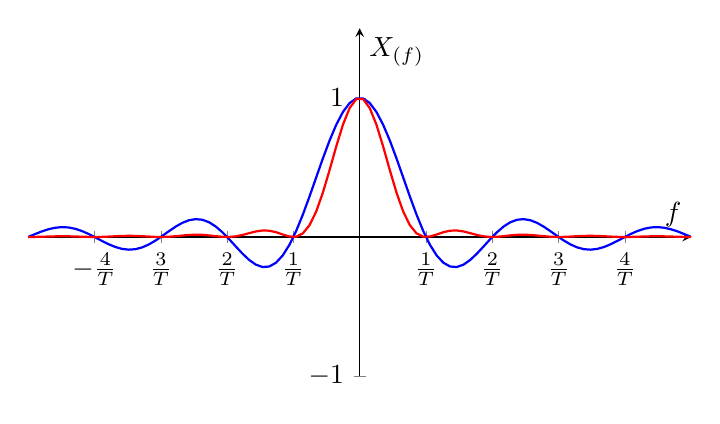
\begin{tikzpicture}
                            \begin{axis}[
                                domain=-5:5,
                                samples=200,
                                axis lines=middle,
                                xlabel=$f$,
                                ylabel=$X_{(f)}$,
                                ytick = {},
                                xtick = {-4,-3,-2,-1,0,1,2,3,4},
                                xticklabels = {$-\frac{4}{T}$,$\frac{3}{T}$,$\frac{2}{T}$,$\frac{1}{T}$,$0$,$\frac{1}{T}$,$\frac{2}{T}$,$\frac{3}{T}$,$\frac{4}{T}$},
                                ymin=-1,
                                ymax=1.5,
                                width=10cm,
                                height=6cm
                            ]
                            \addplot [blue, thick, samples = 100] {sin(deg(x*pi))/(x*pi)};
                            \addplot [red, thick, samples = 100] {(sin(deg(x*pi)))^2/(x*pi)^2};
                            \end{axis}
                        \end{tikzpicture}
                        \caption{{\color{blue}$\frac{sinc}{x}$}, {\color{red}$\frac{sinc^2}{x^2}$}}
                        \label{fig:sinc vs sinc2}
                    \end{figure}
                    DOMANDA: ma la fase in tutto questo che ruolo ha? non avrei problemi avere anche sinc che cambiano la fase degli altri segnali?
                    dopotutto si la sinc é brutta perché si estende all'infinito, ma proprio per questo la fase é sempre sporcata? cosa comporta 
                    nella ricostruzione del segnale? noi abbiamo visto finora l'ampiezza dopotutto
                }
            \end{itemize}
        }
        
        \subsubsection{Derivazione in Frequenza}\label{Derivazione in Frequenza}
            $Ip:\begin{cases}
                x_{(t)}\overunderset{TCF}{ATCF}{\leftrightharpoons} X_{(f)}
                y_{(t)}= \derivative{x_{(t)}}{t}\\        
            \end{cases}$\\
            $Th: Y_{(f)} = j2\pi f X_{(f)} $ \\
            Dimostrazione: ok per ora non l'ha fatta
                
        \subsubsection{Integrazione in Frequenza}\label{Integrazione in Frequenza}
            $Ip:\begin{cases}
                x_{(t)}\overunderset{TCF}{ATCF}{\leftrightharpoons} X_{(f)}
                y_{(t)}= \derivative{x_{(t)}}{t}\\        
            \end{cases}$\\
            $Th: Y_{(f)} = j2\pi f X_{(f)} $ \\
            Dimostrazione: ok per ora non l'ha fatta

                        
        \subsubsection{Convoluzione}\label{Convoluzione}
            \[
                z_{(t)} = x_{(t)} \otimes  y_{(t)} \triangleq \int_{-\infty}^{\infty} x_{(\tau)}y_{(t-\tau)} d\tau
            \] 
            $Ip:\begin{cases}
                x_{(t)}\overunderset{TCF}{ATCF}{\leftrightharpoons} X_{(f)} \\
                x_{(t)}\overunderset{TCF}{ATCF}{\leftrightharpoons} X_{(f)} \\
                z_{(t)} = x_{(t)} \otimes  y_{(t)}   
            \end{cases}$\\
            $Th: Z_{(f)} = X_{(f)}Y_{(f)} $ \\
            Dimostrazione:
                \begin{align}
                    Z_{(f)} &= \int_{-\infty}^{\infty} z_{(t)} e^{-j2\pi ft} dt = \int_{-\infty_{t}}^{\infty}\int_{-\infty_{\tau}}^{\infty} x_{(\tau)}y_{(t-\tau)} e^{-j2\pi ft} dt\ d\tau \nonumber \\
                            &= \int_{-\infty_{t}}^{\infty}x_{(\tau)}\int_{-\infty_{\tau}}^{\infty} y_{(t-\tau)}e^{-j2\pi ft}  dt\ d\tau \overset{Th. \ref{Ritardo}}{\Rightarrow} \int_{-\infty}^{\infty}Y_{(f)}x_{(\tau)}e^{-j2\pi f\tau} d\tau  \nonumber \\
                            &= X_{(f)}Y_{(f)} \nonumber
                \end{align}
            Propietá della convoluzione:
            \begin{itemize}
                \item {
                        Commutativa:
                        \[
                            z_{(t)} = x_{(t)} \otimes  y_{(t)} = y_{(t)} \otimes  x_{(t)}  
                        \]
                        Dimostrazione:
                        \begin{align}
                            z_{(t)} &= \int_{-\infty}^{\infty} x_{(\tau)}y_{(t-\tau)} d\tau \Rightarrow \tau=t-\tau^\prime\Rightarrow \int_{-\infty}^{\infty} x_{(t-\tau^\prime)}y_{(\tau^\prime)} d\tau^\prime \nonumber \\
                                    &= \int_{-\infty}^{\infty} y_{(\tau^\prime)}x_{(t-\tau^\prime)} d\tau^\prime = y_{(t)} \otimes  x_{(t)}\nonumber 
                        \end{align}
                    }\label{Conv. Commutativa}
                \item {
                        Associativa:
                        \[
                            (x_{(t)} \otimes  y_{(t)}) \otimes z_{(t)}  =x_{(t)} \otimes  (y_{(t)} \otimes z_{(t)})   
                        \]
                    }\label{Conv. Distributiva}
                \item {
                        Distributiva:
                        \[
                            x_{(t)} \otimes  (y_{(t)}+z_{(t)}) = x_{(t)}\otimes  y_{(t)} +x_{(t)}\otimes  z_{(t)}  
                        \]
                        Dimostrazione:
                        \begin{align}
                            z_{(t)} &= \int_{-\infty}^{\infty} x_{(\tau)}(y_{(t-\tau)}+z_{(t-\tau)}) d\tau = \int_{-\infty}^{\infty}x_{(\tau)}y_{(t-\tau)} +x_{(\tau)}z_{(t-\tau)} d\tau \nonumber \\
                                    &= \int_{-\infty}^{\infty}x_{(\tau)}y_{(t-\tau)} d\tau +\int_{-\infty}^{\infty}x_{(\tau)}z_{(t-\tau)} d\tau = x_{(t)}\otimes  y_{(t)} +x_{(t)}\otimes  z_{(t)} \nonumber 
                        \end{align}
                    }\label{Conv. Associativa}
            \end{itemize}
            Tutte le propietá sono valutate nel dominio del $tempo$ ma valgono anche per il dominio della $frequenza$.
        \subsubsection{Prodotto}\label{Prodotto}
            $Ip:\begin{cases}
                x_{(t)}\overunderset{TCF}{ATCF}{\leftrightharpoons} X_{(f)} \\
                x_{(t)}\overunderset{TCF}{ATCF}{\leftrightharpoons} X_{(f)} \\
                z_{(t)} = x_{(t)}y_{(t)}   
            \end{cases}$\\
            $Th: Z_{(f)} = X_{(f)}\otimes Y_{(f)} $ \\
            Dimostrazione:
                \begin{align}
                    Z_{(f)} &= \int_{-\infty}^{\infty} z_{(t)} e^{-j2\pi ft} dt = \int_{-\infty}^{\infty}x_{(t)}y_{(t)} e^{-j2\pi ft} dt \nonumber \\
                            &= \int_{-\infty_{t}}^{\infty} \int_{-\infty_{\alpha}}^{\infty}X_{(\alpha)}e^{j2\pi \alpha t} d\alpha\ y_{(t)}e^{-j2\pi ft} dt =\int_{-\infty_{\alpha}}^{\infty}X_{(\alpha)} \int_{-\infty_{t}}^{\infty}y_{(t)}e^{-j2\pi (f-\alpha)t} dt\ d\alpha\nonumber \\
                            &\overset{Th. \ref{Ritardo}}{\Rightarrow} \int_{-\infty}^{\infty}X_{(\alpha)}Y_{(f-\alpha)}  d\alpha = X_{(f)}\otimes Y_{(f)} \nonumber 
                \end{align}
            \begin{align}
                Tempo&\hspace{1cm} Frequenza \nonumber \\ 
                Convoluzione\ &\Longleftrightarrow \ Prodotto \nonumber \\ 
                Prodotto\ &\Longleftrightarrow \ Convoluzione \nonumber 
            \end{align}
        \subsubsection{Calcolo del prodotto di convoluzione}\label{Calcolo del prodotto di convoluzione}
        \[
            x_{(t)} \otimes  y_{(t)} = \int_{-\infty}^{\infty} x_{(\tau)}y_{(t-\tau)} d\tau \hspace{1cm} y_{(-\alpha)}\ e^\prime\ y_{(\alpha)}\ ruotato 
        \]
        Facciamo un esempio con 2 $rect$:\\

        $x_{(t)} = y_{(t)} = rect\left(\frac{t}{T}\right)$
        \begin{figure}[H]
            \centering
            \subfloat[Grafico nel tempo,{\color{red}$y_{(-\alpha)}$},{\color{blue}$x_{(\alpha)}$}]{
                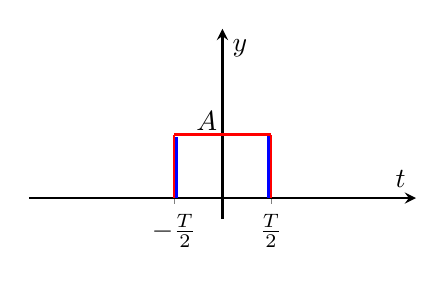
\begin{tikzpicture}
                    \begin{axis}[
                        xlabel=$t$,
                        ylabel=$y$,
                        xmin=-4,
                        xmax=4,
                        ymin=-0.5,
                        ymax=4,
                        ytick = {1.5},
                        xtick={-1, 0, 1},
                        xticklabels={$-\frac{T}{2}$, $0$, $\frac{T}{2}$},
                        yticklabels = {$A$},
                        yticklabel style = {yshift=5pt,xshift=4pt}, 
                        axis lines=middle,
                        thick,
                        domain=-4:4,
                        samples=100,
                        width=6.5cm,
                        height=4cm
                    ]
                    \addplot [const plot, blue, thick] coordinates{(-0.95,1.49)(0.95,1.45)};
                    \addplot [const plot, blue, thick] coordinates{(-0.95,0)(-0.95,1.45)};
                    \addplot [const plot, blue, thick] coordinates{(0.95,0)(0.95,1.45)};
                
                    \addplot [const plot, red, thick] coordinates{(-1,1.5)(1,1.5)};
                    \addplot [const plot, red, thick] coordinates{(-1,0)(-1,1.5)};
                    \addplot [const plot, red, thick] coordinates{(1,0)(1,1.5)};
                
                    \end{axis}
                \end{tikzpicture}
                \label{fig:PC rect}
            }
            \hfill
            \subfloat[illustrazione dell'integrale al variare di $t$,{\color{green}$y_{(t-\alpha)}$},{\color{blue}$x_{(\alpha)}$}]{
                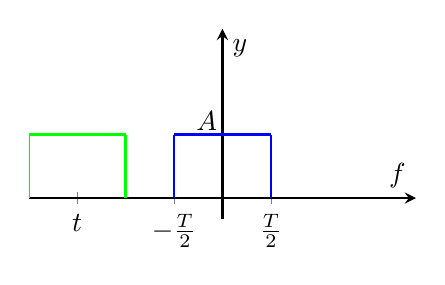
\begin{tikzpicture}
                    \begin{axis}[
                        xlabel=$f$,
                        ylabel=$y$,
                        xmin=-4,
                        xmax=4,
                        ymin=-0.5,
                        ymax=4,
                        ytick = {1.5},
                        xtick={-3,-1, 0, 1},
                        xticklabels={$t$,$-\frac{T}{2}$, $0$, $\frac{T}{2}$},
                        yticklabels = {$A$},
                        yticklabel style = {yshift=5pt,xshift=4pt}, 
                        axis lines=middle,
                        thick,
                        domain=-5:5,
                        samples=100,
                        width=6.5cm,
                        height=4cm
                    ]

                    \addplot [const plot, green, thick] coordinates{(-4,1.5)(-2,1.5)};
                    \addplot [const plot, green, thick] coordinates{(-4,0)(-4,1.5)};
                    \addplot [const plot, green, thick] coordinates{(-2,0)(-2,1.5)};

                    \addplot [const plot, blue, thick] coordinates{(-1,1.5)(1,1.5)};
                    \addplot [const plot, blue, thick] coordinates{(-1,0)(-1,1.5)};
                    \addplot [const plot, blue, thick] coordinates{(1,0)(1,1.5)};
                    \end{axis}
                \end{tikzpicture}
                \label{fig:PC rect in rect}
            }
            \caption{Grafico per il calcolo del prodotto di convoluzione}
        \end{figure}    
        All'aumentare di $t$ {\color{green}$y_{(t-\alpha)}$} si sposta sull'asse delle ascisse, se:
        \begin{itemize}
            \item {
                $t=-\frac{T}{2}$: si allineano le due $rect$ e il valore dell'integrale inizia a aumentare.
            }
            \item {
                $t=0$: si ha il valore massimo del prodotto tra le due funzioni (in questo caso $A=1$), l'integrale vale T.
            }
            \item {
                $t=\frac{T}{2}$: le due $rect$ sono disgiunte, nel raggiungere questa posizione il valore dell'integrale é diminuito fino a $0$.
            }
        \end{itemize}
        Traccamo l'andamento dell'integrale:
        \begin{figure}[H]
            \centering
            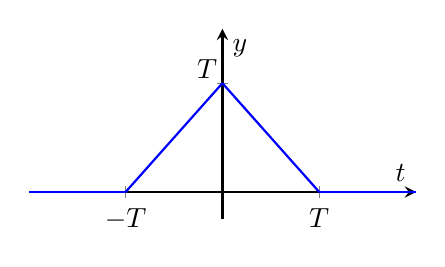
\begin{tikzpicture}
                \begin{axis}[
                    xlabel=$t$,
                    ylabel=$y$,
                    xmin=-4,
                    xmax=4,
                    ymin=-0.5,
                    ymax=3,
                    ytick = {2},
                    xtick={-2, 0, 2},
                    xticklabels={$-T$, $0$, $T$},
                    yticklabels = {$T$},
                    yticklabel style = {yshift=5pt,xshift=4pt}, 
                    axis lines=middle,
                    thick,
                    domain=-4:4,
                    samples=100,
                    width=6.5cm,
                    height=4cm
                ]
                \addplot [sharp plot, blue, thick] coordinates{(-2,0)(0,2)};
                \addplot [sharp plot, blue, thick] coordinates{(2,0)(0,2)};
            
                \addplot [const plot, blue, thick] coordinates{(-2,0)(-4,0)};
                \addplot [const plot, blue, thick] coordinates{(2,0)(4,0)};
            
                \end{axis}
            \end{tikzpicture}
            \label{fig:PC valore integrale}
            \caption{Integrale di convoluzione}
        \end{figure}

        {\em Osservazioni}:
        \begin{itemize}
            \item {Il prodotto di convoluzione ha come durata la somma delle durate dei segnali $[-\frac{T}{2},\frac{T}{2}]\rightarrow[-T,T]$}
            \item {In $t=0$ é l'area il prodotto dei segnali}
        \end{itemize}
        Esempio con $rect$ di durata $T$ e $2T$: 
        \begin{figure}[H]
            \centering
            \subfloat[Grafico delle rect]{
                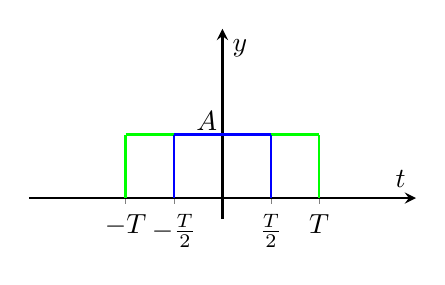
\begin{tikzpicture}
                    \begin{axis}[
                        xlabel=$t$,
                        ylabel=$y$,
                        xmin=-4,
                        xmax=4,
                        ymin=-0.5,
                        ymax=4,
                        ytick = {1.5},
                        xtick={-2,-1, 0, 1,2},
                        xticklabels={$-T$,$-\frac{T}{2}$, $0$, $\frac{T}{2}$,$T$},
                        yticklabels = {$A$},
                        yticklabel style = {yshift=5pt,xshift=4pt}, 
                        axis lines=middle,
                        thick,
                        domain=-4:4,
                        samples=100,
                        width=6.5cm,
                        height=4cm
                    ]
                 
                    \addplot [const plot, green, thick] coordinates{(-2,0)(-2,1.5)};
                    \addplot [const plot, green, thick] coordinates{(2,0)(2,1.5)};
                    \addplot [const plot, green, thick] coordinates{(-2,1.5)(2,1.5)};

                    \addplot [const plot, blue, thick] coordinates{(-1,1.5)(1,1.5)};
                    \addplot [const plot, blue, thick] coordinates{(-1,0)(-1,1.5)};
                    \addplot [const plot, blue, thick] coordinates{(1,0)(1,1.5)};
                    \end{axis}
                \end{tikzpicture}
                \label{fig:PC rect T e 2T}
            }
            \hfill
            \subfloat[Risultato integrale di due $rect$ diverse]{
                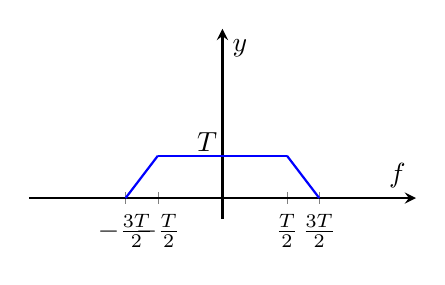
\begin{tikzpicture}
                    \begin{axis}[
                        xlabel=$f$,
                        ylabel=$y$,
                        xmin=-3,
                        xmax=3,
                        ymin=-0.5,
                        ymax=4,
                        ytick = {1},
                        xtick={-3/2,-1, 0,1, 3/2},
                        xticklabels={$-\frac{3T}{2}$,$-\frac{T}{2}$, $0$,$\frac{T}{2}$ ,$\frac{3T}{2}$},
                        yticklabels = {$T$},
                        yticklabel style = {yshift=5pt,xshift=4pt}, 
                        axis lines=middle,
                        thick,
                        domain=-3:3,
                        samples=100,
                        width=6.5cm,
                        height=4cm
                    ]
                        
                    \addplot [sharp plot, blue, thick] coordinates{(-3/2,0)(-1,1)};
                    \addplot [sharp plot, blue, thick] coordinates{(3/2,0)(1,1)};
                    \addplot [sharp plot, blue, thick] coordinates{(-1,1)(1,1)};
                
                    \end{axis}
                \end{tikzpicture}
                \label{fig:PC rect in rect diverse}
            }
            \caption{Integrale di convoluzione di $rect$ di durata diversa}
        \end{figure}
        Esemptio $TCF$ di un triangolo:
        \begin{figure}[H]
            \centering
            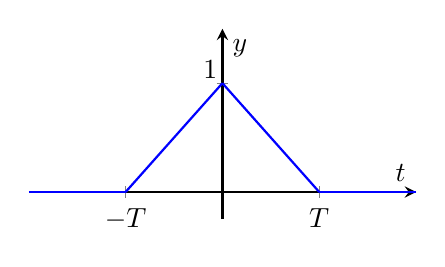
\begin{tikzpicture}
                \begin{axis}[
                    xlabel=$t$,
                    ylabel=$y$,
                    xmin=-4,
                    xmax=4,
                    ymin=-0.5,
                    ymax=3,
                    ytick = {2},
                    xtick={-2, 0, 2},
                    xticklabels={$-T$, $0$, $T$},
                    yticklabels = {$1$},
                    yticklabel style = {yshift=5pt,xshift=4pt}, 
                    axis lines=middle,
                    thick,
                    domain=-4:4,
                    samples=100,
                    width=6.5cm,
                    height=4cm
                ]
                \addplot [sharp plot, blue, thick] coordinates{(-2,0)(0,2)};
                \addplot [sharp plot, blue, thick] coordinates{(2,0)(0,2)};
            
                \addplot [const plot, blue, thick] coordinates{(-2,0)(-4,0)};
                \addplot [const plot, blue, thick] coordinates{(2,0)(4,0)};
            
                \end{axis}
            \end{tikzpicture}
            \label{fig:PC TCF triangolo}
            \caption{Integrale di convoluzione}
        \end{figure}
        Dal Th. di Convoluzione \ref{Convoluzione} sappiamo che é il prodotto di convoluzione di 2 rect di durata uguale a $T$:
        \begin{gather}
            z_{(t)} = x_{(t)}\otimes y_{(t)} = rect\left(\frac{t}{T}\right) \otimes rect\left(\frac{t}{T}\right) \overset{Th. \ref{Convoluzione}}{\Rightarrow} Tsinc(fT)\dotproduct Tsinc(fT) \nonumber \\
            T^2sinc(fT) \nonumber 
        \end{gather}
        Esercizio appunti martorella triangoli a sx a dx:
    \subsection{Modulazione di Ampiezza}\label{Modulazione di Ampiezza}
        % \[
        %     y_{(t)} = x_{(t)}\cos(2\pi f_0t)
        % \]
        \begin{figure}[H]
            \centering
            \subfloat[Sistema di modulazione]{
                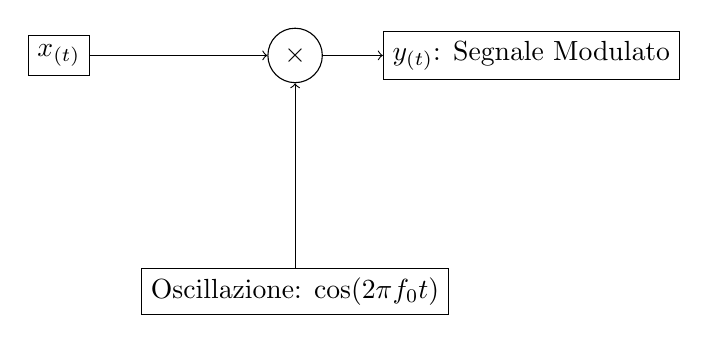
\begin{tikzpicture}[
                        node distance=3cm
                    ]
                    % Blocks
                    \node [rectangle, draw] (input) {$x_{(t)}$};
                    \node [circle, draw, right of=input] (product) {$\times$};
                    \node [rectangle, draw, below of=product] (carrier) {Oscillazione: $\cos(2\pi f_0t)$};
                    \node [rectangle, draw, right of=product] (modulated) {$y_{(t)}$: Segnale Modulato};
                
                    % Connections
                    \draw [->] (input) -- (product);
                    \draw [->] (product) -- (modulated);
                    \draw [->] (carrier) -- (product);
                \end{tikzpicture}    
                \label{fig:sistema di modulazione}
            }
            \hfill
            \subfloat[{\color{blue}$x_{(t)}$}, {\color{red}$y_{(t)}$}, {\color{purple}$\cos (2\pi t)$}]{
                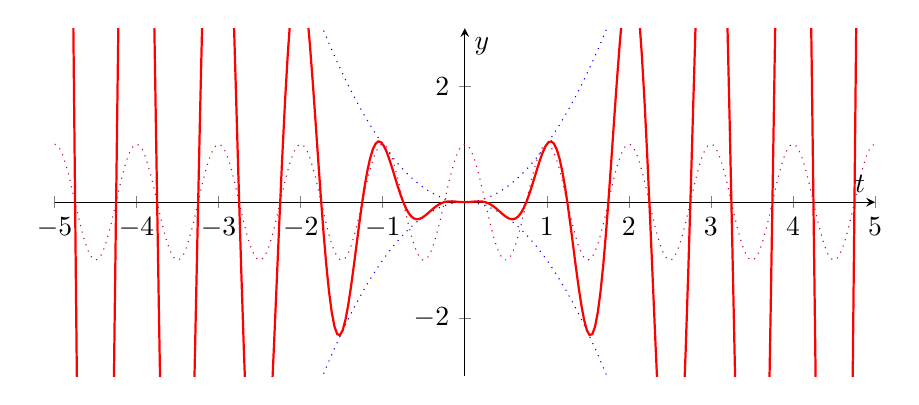
\begin{tikzpicture}
                    \begin{axis}[
                        domain=-5:5,
                        samples=200,
                        axis lines=middle,
                        xlabel=$t$,
                        ylabel=$y$,
                        ymin=-3,
                        ymax=3,
                        width=12cm,
                        height=6cm
                    ]
                    \addplot [blue, dotted, samples = 300] {(x^2)};
                    \addplot [blue, dotted, samples = 300] {-(x^2)};
                    \addplot [purple,dotted, samples = 300] {cos(deg(2*pi*x))};
                    \addplot [red, thick, samples = 300] {cos(deg(2*pi*x))*(x^2)};
                    \end{axis}
                \end{tikzpicture}
                \label{fig:modulazione in ampiezza}
            }
            \caption{Esempio sistema di modulazione di ampiezza}
        \end{figure}
        L'oscillazione introdotta, $\cos (2\pi t)$, segue l'andamento di $x_{(t)}$
        Nel dominio della frequenza:
        \begin{figure}[H]
            \centering
            \subfloat[Senza modulazione]{
                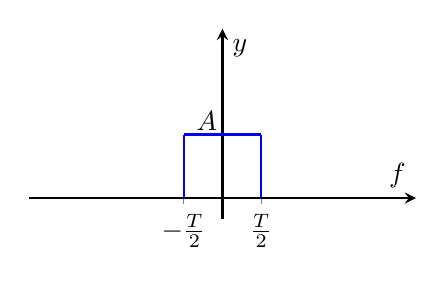
\begin{tikzpicture}
                    \begin{axis}[
                        xlabel=$f$,
                        ylabel=$y$,
                        xmin=-5,
                        xmax=5,
                        ymin=-0.5,
                        ymax=4,
                        ytick = {1.5},
                        xtick={-1, 0, 1},
                        xticklabels={$-\frac{T}{2}$, $0$, $\frac{T}{2}$},
                        yticklabels = {$A$},
                        yticklabel style = {yshift=5pt,xshift=4pt}, 
                        axis lines=middle,
                        thick,
                        domain=-5:5,
                        samples=100,
                        width=6.5cm,
                        height=4cm
                    ]
                    \addplot [const plot, blue, thick] coordinates{(-1,1.5)(1,1.5)};
                    \addplot [const plot, blue, thick] coordinates{(-1,0)(-1,1.5)};
                    \addplot [const plot, blue, thick] coordinates{(1,0)(1,1.5)};
                
                    \end{axis}
                \end{tikzpicture}
                \label{fig:segnale senza modulazione}
            }
            \hfill
            \subfloat[Con modulazione]{
                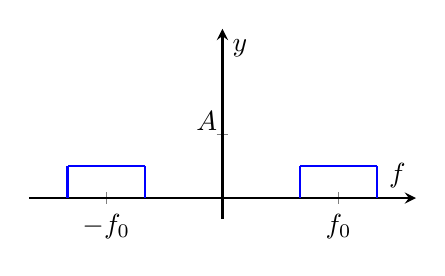
\begin{tikzpicture}
                    \begin{axis}[
                        xlabel=$f$,
                        ylabel=$y$,
                        xmin=-5,
                        xmax=5,
                        ymin=-0.5,
                        ymax=4,
                        ytick = {1.5},
                        xtick={-3,0,3},
                        xticklabels={$-f_0$, $0$,$f_0$},
                        yticklabels = {$A$},
                        yticklabel style = {yshift=5pt,xshift=4pt}, 
                        axis lines=middle,
                        thick,
                        domain=-5:5,
                        samples=100,
                        width=6.5cm,
                        height=4cm
                    ]
                    \addplot [const plot, blue, thick] coordinates{(-2,0.75)(-4,0.75)};
                    \addplot [const plot, blue, thick] coordinates{(-2,0)(-2,0.75)};
                    \addplot [const plot, blue, thick] coordinates{(-4,0)(-4,0.75)};
                    
                    \addplot [const plot, blue, thick] coordinates{(2,0.75)(4,0.75)};
                    \addplot [const plot, blue, thick] coordinates{(2,0)(2,0.75)};
                    \addplot [const plot, blue, thick] coordinates{(4,0)(4,0.75)};
                    
                    \end{axis}
                \end{tikzpicture}
                \label{fig:segnale con modulazione}
            }
            \caption{Segnale nel dominio della frequenza modulato e non}
        \end{figure}
        Serve per spostare la frequenza (es. di trasmissione) del segnale in modo tale, ad esempio, da non sovrapporre due segnali che sono sulla stessa frequenza.
        Se il segnale non fosse modulato si dice in {\color{blue} \textbf{banda base} (BB)} se il segnale é modulato si dice in {\color{red}\textbf{banda passante}(BP)}.
        \begin{figure}[H]
            \centering
            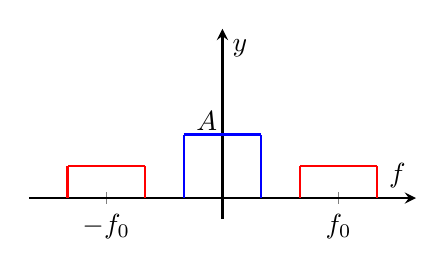
\begin{tikzpicture}
                \begin{axis}[
                    xlabel=$f$,
                    ylabel=$y$,
                    xmin=-5,
                    xmax=5,
                    ymin=-0.5,
                    ymax=4,
                    ytick = {1.5},
                    xtick={-3,0,3},
                    xticklabels={$-f_0$, $0$,$f_0$},
                    yticklabels = {$A$},
                    yticklabel style = {yshift=5pt,xshift=4pt}, 
                    axis lines=middle,
                    thick,
                    domain=-5:5,
                    samples=100,
                    width=6.5cm,
                    height=4cm
                ]
                \addplot [const plot, red, thick] coordinates{(-2,0.75)(-4,0.75)};
                \addplot [const plot, red, thick] coordinates{(-2,0)(-2,0.75)};
                \addplot [const plot, red, thick] coordinates{(-4,0)(-4,0.75)};
                
                \addplot [const plot, red, thick] coordinates{(2,0.75)(4,0.75)};
                \addplot [const plot, red, thick] coordinates{(2,0)(2,0.75)};
                \addplot [const plot, red, thick] coordinates{(4,0)(4,0.75)};
            
                \addplot [const plot, blue, thick] coordinates{(-1,1.5)(1,1.5)};
                \addplot [const plot, blue, thick] coordinates{(-1,0)(-1,1.5)};
                \addplot [const plot, blue, thick] coordinates{(1,0)(1,1.5)};
            
                
                \end{axis}
            \end{tikzpicture}
            \caption{{\color{blue}BB}, {\color{red}BP}}
            \label{fig:bb e bp}
        \end{figure}

        \subsubsection{Th. Modulazione con $\cos(2\pi f_0t)$}\label{Modulazione con coseno}
            $Ip:\begin{cases}
                    y_{(t)}= x_{(t)}\cos(2\pi f_0t)\\        
                    x_{(t)}\overunderset{TCF}{ATCF}{\leftrightharpoons} X_{(f)}
                \end{cases}$\\
            $Th: Y_{(f)} = \frac{1}{2} X_{(f-f_0)} + \frac{1}{2} X_{(f+f_0)}$ \\
            Dimostrazione:
            \begin{align}
                Y_{(f)} & = \int_{-\infty}^{\infty} y_{(t)} e^{-j2\pi ft} dt = \int_{-\infty}^{\infty} x_{(t)}\cos(2\pi f_0t) e^{-j2\pi ft} dt \nonumber \\
                & =\int_{-\infty}^{\infty} x_{(t)} \frac{e^{j2\pi f_0t} + e^{-j2\pi f_0t}}{2} e^{-j2\pi ft} dt =  \nonumber \\
                & = \frac{1}{2} \int_{-\infty}^{\infty} x_{(t)} e^{-j2\pi (f-f_0)t} dt + \frac{1}{2} \int_{-\infty}^{\infty} x_{(t)} e^{-j2\pi (f+f_0)t} dt \nonumber \\
                & = \eval{TCF[x_{(t)}]}_{f-f_0} + \eval{TCF[x_{(t)}]}_{f+f_0} = \frac{1}{2} X_{(f-f_0)} + \frac{1}{2} X_{(f+f_0)}\ c.v.d \nonumber  
            \end{align}
            Esempio:\\
            {
                $X_{(f)} = \frac{A}{B}rect\left(\frac{f}{B}\right)$
                \[
                    Y_{(f)} = \frac{A}{2B}rect\left(\frac{f-f_0}{B}\right)+\frac{A}{2B}rect\left(\frac{f+f_0}{B}\right)
                \]
                \begin{figure}[H]
                    \centering
                    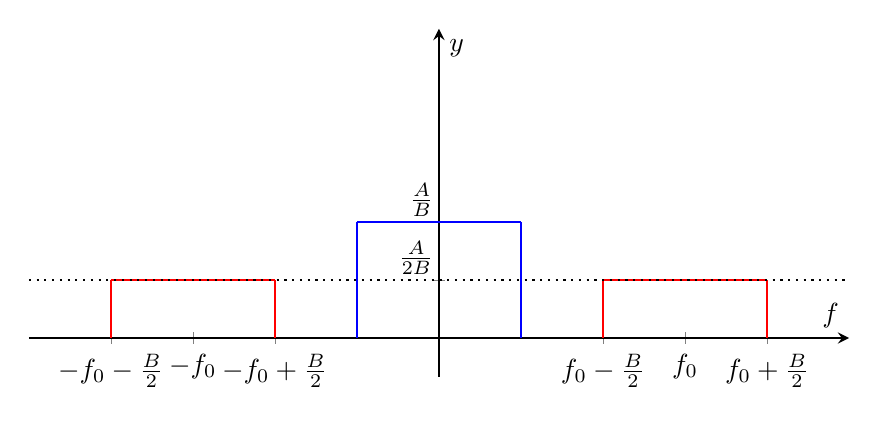
\begin{tikzpicture}
                        \begin{axis}[
                            xlabel=$f$,
                            ylabel=$y$,
                            xmin=-5,
                            xmax=5,
                            ymin=-0.5,
                            ymax=4,
                            ytick = {0.75,1.5},
                            xtick={-4,-3,-2, 0,2,3,4},
                            xticklabels={$-f_0-\frac{B}{2}$,$-f_0$,$-f_0+\frac{B}{2}$,$0$,$f_0-\frac{B}{2}$,$f_0$,$f_0+\frac{B}{2}$},
                            yticklabels = {$\frac{A}{2B}$,$\frac{A}{B}$},
                            yticklabel style = {yshift=8pt,xshift=4pt}, 
                            axis lines=middle,
                            thick,
                            domain=-5:5,
                            samples=100,
                            width=12cm,
                            height=6cm
                        ]
                        \addplot [const plot, red, thick] coordinates{(-2,0.75)(-4,0.75)};
                        \addplot [const plot, red, thick] coordinates{(-2,0)(-2,0.75)};
                        \addplot [const plot, red, thick] coordinates{(-4,0)(-4,0.75)};
                        
                        \addplot [const plot, red, thick] coordinates{(2,0.75)(4,0.75)};
                        \addplot [const plot, red, thick] coordinates{(2,0)(2,0.75)};
                        \addplot [const plot, red, thick] coordinates{(4,0)(4,0.75)};
                    
                        \addplot [const plot, blue] coordinates{(-1,1.5)(1,1.5)};
                        \addplot [const plot, blue] coordinates{(-1,0)(-1,1.5)};
                        \addplot [const plot, blue] coordinates{(1,0)(1,1.5)};
                        
                        \addplot [const plot,dotted, black] coordinates{(-5,0.75)(5,0.75)};

                        \end{axis}
                    \end{tikzpicture}
                    \caption{{\color{blue}$X_{(f)}$}, {\color{red}$Y_{(f)}$}}
                    \label{fig:modulazione rect}
                \end{figure}
            }
        \subsubsection{Th. Modulazione con $\sin(2\pi f_0t)$}\label{Modulazione con seno}
        $Ip:\begin{cases}
                y_{(t)}= x_{(t)}\sin(2\pi f_0t)\\        
                x_{(t)}\overunderset{TCF}{ATCF}{\leftrightharpoons} X_{(f)}
            \end{cases}$\\
        $Th: Y_{(f)} = \frac{1}{2j} X_{(f-f_0)} - \frac{1}{2j} X_{(f+f_0)} $ \\
        Dimostrazione: 
        \begin{align}
            Y_{(f)} & = \int_{-\infty}^{\infty} y_{(t)} e^{-j2\pi ft} dt = \int_{-\infty}^{\infty} x_{(t)}\sin(2\pi f_0t) e^{-j2\pi ft} dt \nonumber \\
            & =\int_{-\infty}^{\infty} x_{(t)} \frac{e^{j2\pi f_0t} - e^{-j2\pi f_0t}}{2j} e^{-j2\pi ft} dt =  \nonumber \\
            & = \frac{1}{2j} \int_{-\infty}^{\infty} x_{(t)} e^{-j2\pi (f-f_0)t} dt - \frac{1}{2j} \int_{-\infty}^{\infty} x_{(t)} e^{-j2\pi (f+f_0)t} dt \nonumber \\
            & = \eval{TCF[x_{(t)}]}_{f-f_0} - \eval{TCF[x_{(t)}]}_{f+f_0} = \frac{1}{2j} X_{(f-f_0)} - \frac{1}{2j} X_{(f+f_0)}\ c.v.d \nonumber  
        \end{align}

        \subsubsection{Th. Modulazione con $\cos(2\pi f_0t + \phi)$}\label{Modulazione con coseno generico}
            $Ip: \begin{cases}
                y_{(t)}= x_{(t)}\cos(2\pi f_0t + \phi)\\        
                x_{(t)}\overunderset{TCF}{ATCF}{\leftrightharpoons} X_{(f)}
                \end{cases}$\\
            $Th: Y_{(f)} = \frac{e^{j\phi}}{2} X_{(f-f_0)} + \frac{e^{-j\phi}}{2} X_{(f+f_0)} $ \\
            Dimostrazione: 
            \begin{align}
                Y_{(f)} & = \int_{-\infty}^{\infty} y_{(t)} e^{-j2\pi ft} dt = \int_{-\infty}^{\infty} x_{(t)}\cos(2\pi f_0t + \phi) e^{-j2\pi ft} dt \nonumber \\
                & =\int_{-\infty}^{\infty} x_{(t)} \frac{e^{j(2\pi f_0t+ \phi)} + e^{-j(2\pi f_0t+ \phi)}}{2} e^{-j2\pi ft} dt =  \nonumber \\
                & = \frac{e^{j\phi}}{2} \int_{-\infty}^{\infty} x_{(t)} e^{-j2\pi (f-f_0)t} dt + \frac{e^{-j\phi}}{2} \int_{-\infty}^{\infty} x_{(t)} e^{-j2\pi (f+f_0)t} dt \nonumber \\
                & = \eval{TCF[x_{(t)}]}_{f-f_0} + \eval{TCF[x_{(t)}]}_{f+f_0} = \frac{e^{j\phi}}{2} X_{(f-f_0)} + \frac{e^{-j\phi}}{2} X_{(f+f_0)}\ c.v.d \nonumber  
            \end{align}
            Esempio:
            \begin{figure}[H]
                \centering
                \subfloat[Ampiezza Mod. generica]{
                    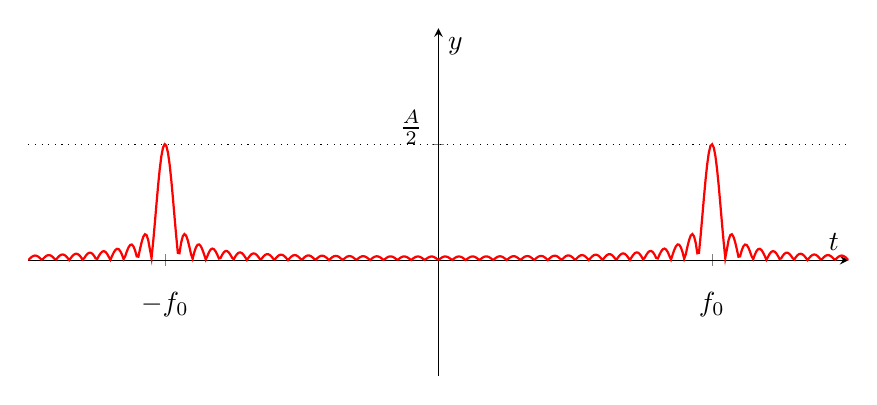
\begin{tikzpicture}
                        \begin{axis}[
                            domain=-30:30,
                            samples=200,
                            axis lines=middle,
                            xlabel=$t$,
                            ylabel=$y$,
                            ytick = {0.5},
                            yticklabels = {$\frac{A}{2}$},
                            yticklabel style = {yshift=6pt},
                            xtick = {-20,20},
                            xticklabels = {$-f_0$,$f_0$},
                            xticklabel style = {yshift=-6pt}, 
                            ymin=-0.5,
                            ymax=1,
                            width=12cm,
                            height=6cm
                        ]
                        \addplot [const plot, dotted,black] coordinates{(-30,0.5)(30,0.5)};
                        \addplot [red, thick, samples = 500] {abs(sin(deg((x-20)*pi))/(2*(x-20)*pi))+abs(sin(deg((x+20)*pi))/(2*(x+20)*pi))};
                        % \addplot [red, thick, samples = 500] {abs(sin(deg((x+20)*pi))/(2*(x+20)*pi))};
                        \end{axis}
                    \end{tikzpicture}
                    \label{fig:Ampiezza Mod. generica}
                }
                \hfill
                \subfloat[fase Mod. generica]{
                        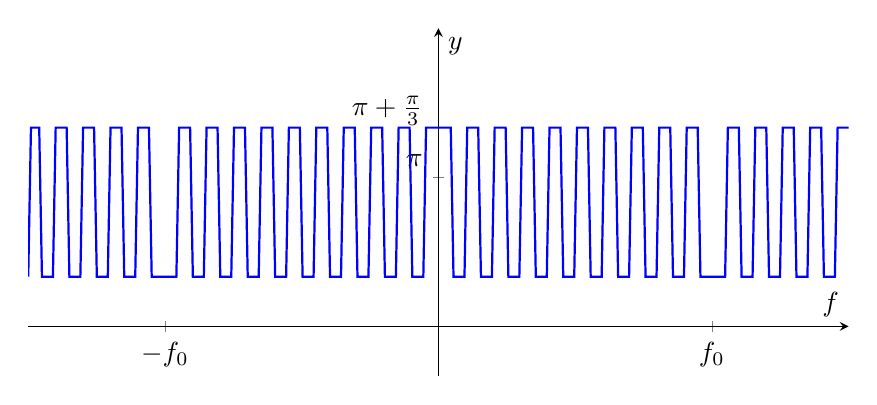
\begin{tikzpicture}
                            \begin{axis}[
                                domain=-30:30,
                                samples=200,
                                axis lines=middle,
                                xlabel=$f$,
                                ylabel=$y$,
                                ymin=-pi/3,
                                ymax=2*pi,
                                xtick={-20,20},
                                xticklabels={$-f_0$,$f_0$},
                                ytick={pi,pi+(pi*1/3)},
                                yticklabel style = {yshift=6pt}, 
                                yticklabels={$\pi$,$\pi+\frac{\pi}{3} $},
                                width=12cm,
                                height=6cm
                            ]
                            \addplot [blue, thick, samples = 300] {rad(atan2(0,(x*sin(deg(pi*x)))/(pi*(-400 + x^2))))+(pi*1/3)};
                            \end{axis}
                        \end{tikzpicture}
                    \label{fig:fase Mod. generica}
                }
                \caption{Modulazione generica di una $A rect\left(\frac{t}{T}\right)$ con $\cos(2\pi f_0t+\frac{\pi}{3})$}
            \end{figure}
        É legale cosa ho scritto sopra della modulazione generica?
        \subsubsection{Th. Modulazione con Esponenziale Complesso}\label{Modulazione con Esponenziale Complesso}
            $Ip: \begin{cases}
                y_{(t)}= x_{(t)}e^{j2\pi f_0t}\\        
                x_{(t)}\overunderset{TCF}{ATCF}{\leftrightharpoons} X_{(f)}
                \end{cases}$\\
            $Th: Y_{(f)} = X_{(f-f_0)} $ \\
            Dimostrazione: 
            \begin{align}
                Y_{(f)} & = \int_{-\infty}^{\infty} y_{(t)} e^{-j2\pi ft} dt = \int_{-\infty}^{\infty} x_{(t)}e^{j2\pi f_0t} e^{-j2\pi ft} dt \nonumber \\
                & =\int_{-\infty}^{\infty} x_{(t)} e^{-j2\pi (f-f_0)t} dt = \eval{TCF[x_{(t)}]}_{f-f_0} = X_{(f-f_0)} \nonumber
            \end{align}
            Posso notare che:
            \begin{itemize}
                \item Ritardo: $\rightarrow x_{(t-t_0)} \rightleftharpoons X_{(f)} e^{(-j2\pi ft_0)}$
                \item Modulazione: $\rightarrow x_{(t)}e^{(j2\pi f_0t)} \rightleftharpoons X_{(f-f_0)}$
            \end{itemize}
            Procedimento per la sintesi di un segnale:
            \begin{itemize}
                \item Derivo il segnale
                \item Verifico le ipotesi del Th. dell'Integrazione \ref{Integrazione}
                \item calcolo la TCF della derivata
                \item Applico il Th. dell'integrazione per calcolare $X_{(f)}$
            \end{itemize}

            \subsubsection{Demodulazione}\label{Demodulazione}
            Ci poniamo il problema di riportare il segnale modulato al segnale originale($g_{(t)}$), dato:\\
            $x_{(t)} = g_{(t)} \cos(2\pi f_0t)$\\
            Demoduliamo il segnale con $2\cos(2\pi f_0t)$:
            \begin{align}
                y_{(t)} &= x_{(t)} {\color{purple}2}\cos(2\pi f_0t) = g_{(t)} \cos^2(2\pi f_0t) \nonumber \\
                        &= g_{(t)} \frac{1+ \cos(4\pi f_0t)}{2} = \frac{g_{(t)}}{2} + \frac{g_{(t)}\cos(4\pi f_0t)}{2}\nonumber\\
                TCF[y_{(t)}] &\overset{Th. \ref{Modulazione con coseno}}{\Rightarrow}  \frac{2G_{(f)}}{2} + \frac{2G_{(f-2f_0)}}{2}+ \frac{2G_{(f+2f_0)}}{2} \nonumber \\
                        &= G_{(f)}+G_{(f-2f_0)}+G_{(f+2f_0)}
            \end{align}
            Dall'ultima uguagliaza posso quindi usare un filtro in ({\color{blue}BB}) per rimuovere i segnali alle frequenze $\pm 2f_0$ e ricavare il mio segnale $G_{(f)}$.\\
            DOMANDA: posso anche quindi demodulare con un seno tanto non mi interessa quello che succede alle frequenze spostate,
            quindi peró ritorno sulla fase, non é importante? usando un seno la ribalto praticamente no? ricontroll cio che stai dicendo bro non so 
            se é giusto il ribaltamento \\
            ALTRA DOMANDA: devo anche modulare il segnale abbastanza lontano dalla BB sennó quando demodulo mi autodisturbo il segnale? da qui deriva $\frac{1}{T}<2BB$\\
            ALTRA DOMANDA: quindi se volessi captare piú segnali mi conviene utilizzare circuiti diversi? oppure posso modulare e demodulare a piacimento i segnali tenendo conto 
            su quali frequenze ho modulato in modo tale da sapere dove vanno a finire i segnali e recuperarli? tanto non mi interessa su quale frequenza finiscano finche non diventino 
            non recuperabili per sovrapposizione giusto?\\
            Riporto un po di esempi di demodulazione di una o piú $rect$:
            Esempio di Demodulazione
            \begin{figure}[H]
                \centering
                \subfloat[$sinc$ modulata]{
                    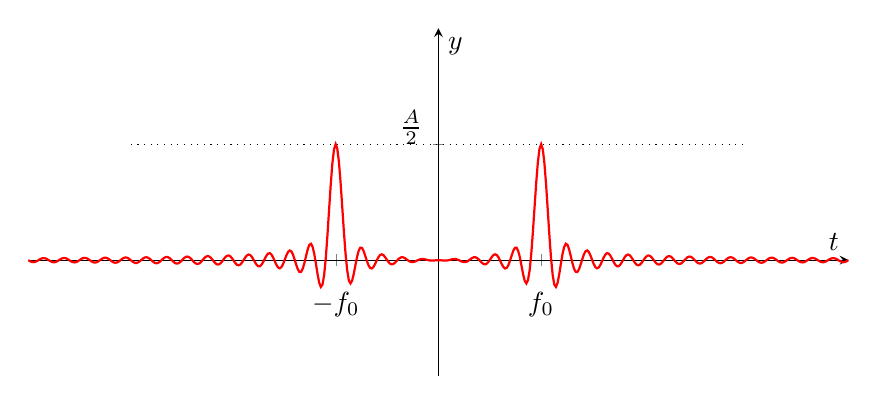
\begin{tikzpicture}
                        \begin{axis}[
                            domain=-40:40,
                            samples=200,
                            axis lines=middle,
                            xlabel=$t$,
                            ylabel=$y$,
                            ytick = {0.5},
                            yticklabels = {$\frac{A}{2}$},
                            yticklabel style = {yshift=6pt},
                            xtick = {-10,10},
                            xticklabels = {$-f_0$,$f_0$},
                            xticklabel style = {yshift=-6pt}, 
                            ymin=-0.5,
                            ymax=1,
                            width=12cm,
                            height=6cm
                        ]
                        \addplot [const plot, dotted,black] coordinates{(-30,0.5)(30,0.5)};
                        \addplot [red, thick, samples = 500] {(sin(deg((x-10)*pi))/(2*(x-10)*pi))+(sin(deg((x+10)*pi))/(2*(x+10)*pi))};
                        \end{axis}
                    \end{tikzpicture}
                    \label{fig:sinc modulata}
                }
                \hfill
                \subfloat[$sinc$ demodulata]{
                    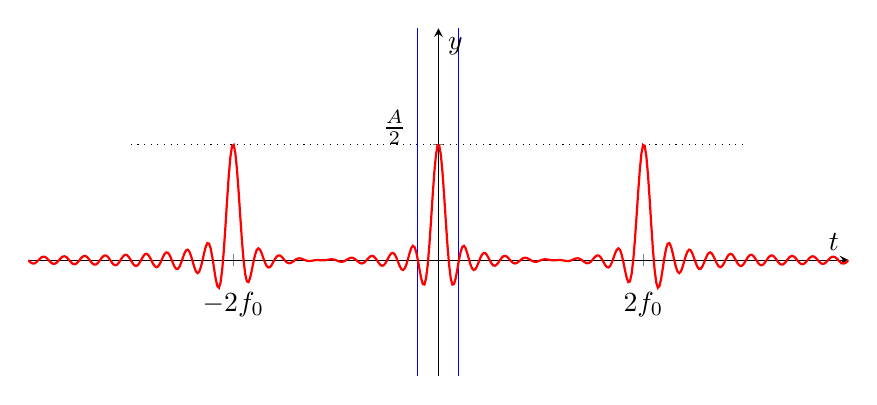
\begin{tikzpicture}
                        \begin{axis}[
                            domain=-40:40,
                            samples=200,
                            axis lines=middle,
                            xlabel=$t$,
                            ylabel=$y$,
                            ytick = {0.5},
                            yticklabels = {$\frac{A}{2}$},
                            yticklabel style = {yshift=6pt,xshift=-6pt},
                            xtick = {-20,20},
                            xticklabels = {$-2f_0$,$2f_0$},
                            xticklabel style = {yshift=-6pt}, 
                            ymin=-0.5,
                            ymax=1,
                            width=12cm,
                            height=6cm
                        ]
                        \addplot [const plot, dotted,black] coordinates{(-30,0.5)(30,0.5)};
                        \addplot [const plot,blue] coordinates{(-2,-0.5)(-2,1)};
                        \addplot [const plot,blue] coordinates{(2,-0.5)(2,1)};
                        \addplot [red, thick, samples = 500] {(sin(deg((x)*pi))/(2*(x)*pi))+(sin(deg((x-20)*pi))/(2*(x-20)*pi))+(sin(deg((x+20)*pi))/(2*(x+20)*pi))};
                        \end{axis}
                    \end{tikzpicture}
                    \label{fig:demodulazione di una sinc}
                }
                \caption{Demodulazione di una $sinc$}
            \end{figure}
            Nel caso di piú segnali durante la demodulazione il segnale che voglio recuperare viene spostato in {\color{blue}BB}
            mentre gli altri segnali presenti sullo spettro vengono a loro volta modulati peró con un $f_0$ diverso rispetto al loro $f_0^\prime$:
            \begin{figure}[H]
                \centering
                \subfloat[Due $sinc$ modulate]{
                    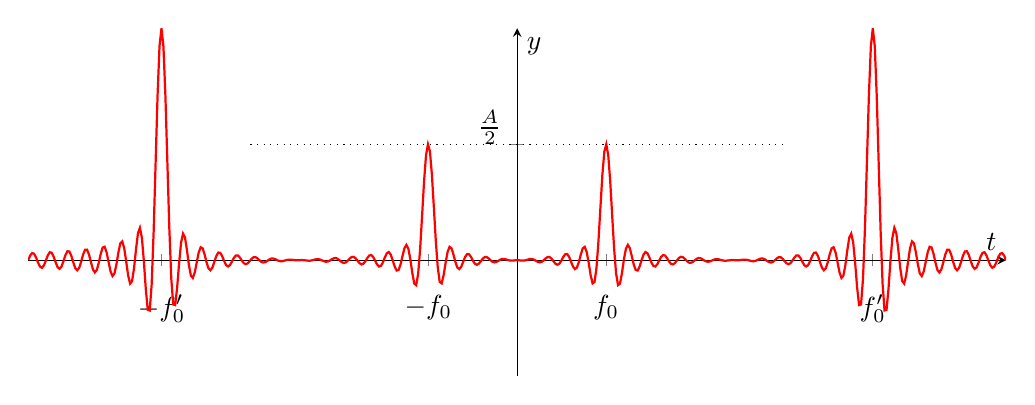
\begin{tikzpicture}
                        \begin{axis}[
                            domain=-55:55,
                            samples=200,
                            axis lines=middle,
                            xlabel=$t$,
                            ylabel=$y$,
                            ytick = {0.5},
                            yticklabels = {$\frac{A}{2}$},
                            yticklabel style = {yshift=6pt},
                            xtick = {-40,-10,10,40},
                            xticklabels = {$-f_0^\prime$,$-f_0$,$f_0$,$f_0^\prime$},
                            xticklabel style = {yshift=-7pt}, 
                            ymin=-0.5,
                            ymax=1,
                            width=14cm,
                            height=6cm
                        ]
                        \addplot [const plot, dotted,black] coordinates{(-30,0.5)(30,0.5)};
                        \addplot [red, thick, samples = 500] {(sin(deg((x-10)*pi))/(2*(x-10)*pi))+(sin(deg((x+10)*pi))/(2*(x+10)*pi))+(sin(deg((x-40)*pi))/((x-40)*pi))+(sin(deg((x+40)*pi))/((x+40)*pi))};
                        \end{axis}
                    \end{tikzpicture}
                    \label{fig:due sinc modulate}
                }
                \hfill
                \subfloat[Demodulazione delle $sinc$]{
                    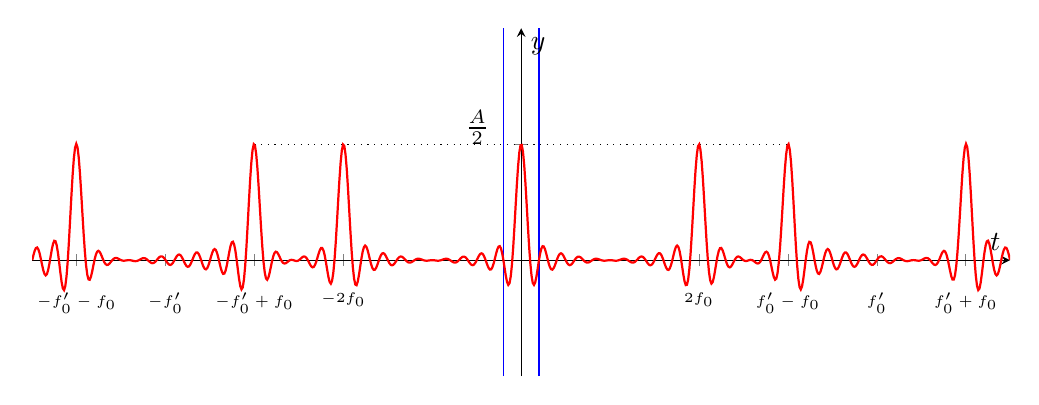
\begin{tikzpicture}
                        \begin{axis}[
                            domain=-55:55,
                            samples=200,
                            axis lines=middle,
                            xlabel=$t$,
                            ylabel=$y$,
                            ytick = {0.5},
                            yticklabels = {$\frac{A}{2}$},
                            yticklabel style = {yshift=6pt,xshift=-6pt},
                            xtick = {-50,-40,-30,-20,20,30,40,50},
                            xticklabels = {$-f_0^\prime-f_0$,$-f_0^\prime$,$-f_0^\prime+f_0$,$-2f_0$,$2f_0$,$f_0^\prime-f_0$,$f_0^\prime$,$f_0^\prime+f_0$},
                            xticklabel style = {yshift=-6pt,font=\tiny}, 
                            ymin=-0.5,
                            ymax=1,
                            width=14cm,
                            height=6cm
                        ]
                        \addplot [const plot, dotted,black] coordinates{(-30,0.5)(30,0.5)};
                        \addplot [const plot,blue] coordinates{(-2,-0.5)(-2,1)};
                        \addplot [const plot,blue] coordinates{(2,-0.5)(2,1)};
                        \addplot [red, thick, samples = 800] {(sin(deg((x)*pi))/(2*(x)*pi))+(sin(deg((x-20)*pi))/(2*(x-20)*pi))+(sin(deg((x+20)*pi))/(2*(x+20)*pi))+(sin(deg((x-50)*pi))/(2*(x-50)*pi))+(sin(deg((x-30)*pi))/(2*(x-30)*pi))+(sin(deg((x+50)*pi))/(2*(x+50)*pi))+(sin(deg((x+30)*pi))/(2*(x+30)*pi))};
                        \end{axis}
                    \end{tikzpicture}
                    \label{fig:demodulazione di due sinc}
                }
                \caption{Demodulazione di due $sinc$}
            \end{figure}
            Potrei peró trovarmi in situazioni delle quali non posso recuperare il segnale
            \begin{figure}[H]
                \centering
                \subfloat[Due $sinc$ modulate]{
                    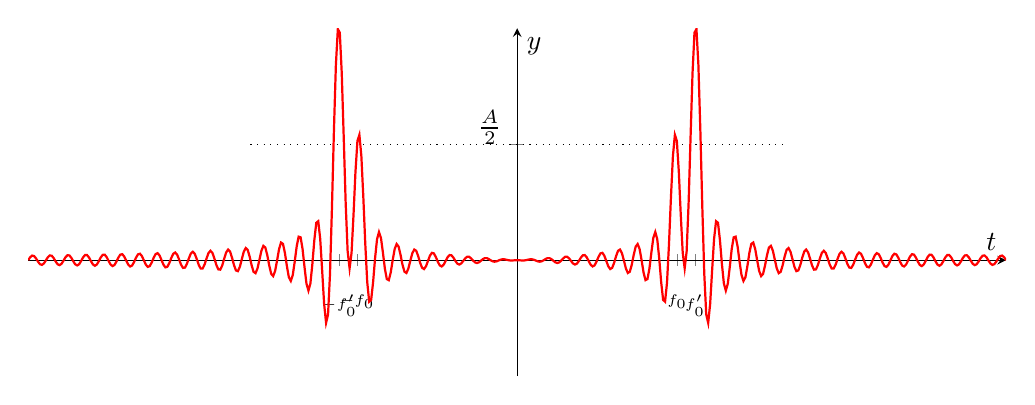
\begin{tikzpicture}
                        \begin{axis}[
                            domain=-55:55,
                            samples=200,
                            axis lines=middle,
                            xlabel=$t$,
                            ylabel=$y$,
                            ytick = {0.5},
                            yticklabels = {$\frac{A}{2}$},
                            yticklabel style = {yshift=6pt},
                            xtick = {-20,-18,18,20},
                            xticklabels = {$-f_0^\prime$,$-f_0$,$f_0$,$f_0^\prime$},
                            xticklabel style = {yshift=-7pt,font=\tiny}, 
                            ymin=-0.5,
                            ymax=1,
                            width=14cm,
                            height=6cm
                        ]
                        \addplot [const plot, dotted,black] coordinates{(-30,0.5)(30,0.5)};
                        \addplot [red, thick, samples = 500] {(sin(deg((x-18)*pi))/(2*(x-18)*pi))+(sin(deg((x+18)*pi))/(2*(x+18)*pi))+(sin(deg((x-20)*pi))/((x-20)*pi))+(sin(deg((x+20)*pi))/((x+20)*pi))};
                        \end{axis}
                    \end{tikzpicture}
                    \label{fig:sinc non recuperabile}
                }
                \hfill
                \subfloat[Demodulazione delle $sinc$]{
                    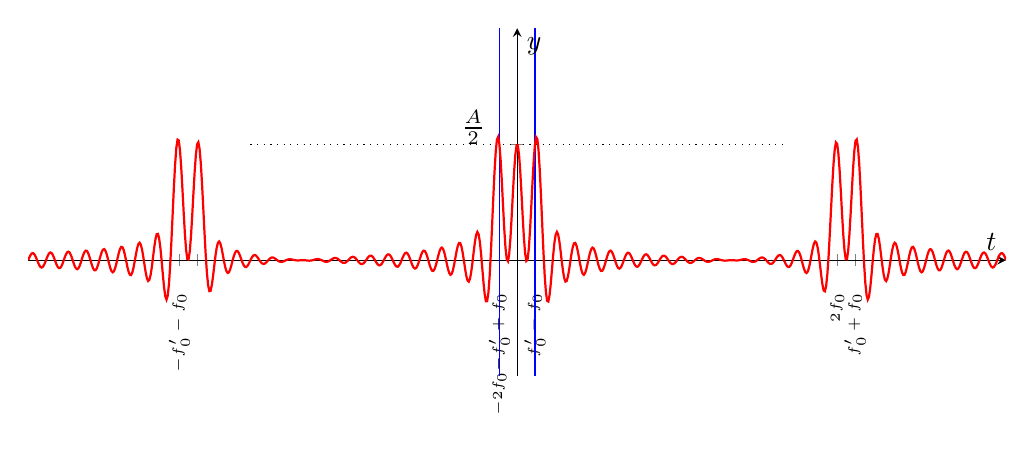
\begin{tikzpicture}
                        \begin{axis}[
                            domain=-55:55,
                            samples=200,
                            axis lines=middle,
                            xlabel=$t$,
                            ylabel=$y$,
                            ytick = {0.5},
                            yticklabels = {$\frac{A}{2}$},
                            yticklabel style = {yshift=6pt,xshift=-6pt},
                            xtick = {-38,-36,-2,2,36,38},
                            xticklabels = {$-f_0^\prime-f_0$,,$-2f_0$$-f_0^\prime+f_0$,$f_0^\prime-f_0$,$2f_0$,$f_0^\prime+f_0$},
                            xticklabel style = {yshift=-6pt,font=\tiny,rotate=90}, 
                            ymin=-0.5,
                            ymax=1,
                            width=14cm,
                            height=6cm
                        ]
                        \addplot [const plot, dotted,black] coordinates{(-30,0.5)(30,0.5)};
                        \addplot [const plot,blue] coordinates{(-2,-0.5)(-2,1)};
                        \addplot [const plot,blue] coordinates{(2,-0.5)(2,1)};
                        \addplot [red, thick, samples = 800] {(sin(deg((x)*pi))/(2*(x)*pi))+(sin(deg((x-36)*pi))/(2*(x-36)*pi))+(sin(deg((x+36)*pi))/(2*(x+36)*pi))+(sin(deg((x-38)*pi))/(2*(x-38)*pi))+(sin(deg((x-2)*pi))/(2*(x-2)*pi))+(sin(deg((x+38)*pi))/(2*(x+38)*pi))+(sin(deg((x+2)*pi))/(2*(x+2)*pi))};
                        \end{axis}
                    \end{tikzpicture}
                    \label{fig:demodulazione sinc non recuperabile}
                }
                \caption{Demodulazione di due $sinc$ non recuperabili}
            \end{figure}
            Come possiamo vedere nella regione della {\color{blue}BB}, il segnale é molto sporco, magari puó essere confuso con un 
            $\cos$ e non una sinc. inoltre ora qui ho usato numeri interi per fare il $plot$ quindi non si accavallano cosí male 
            ma si accavallano solo in $\frac{1}{T}$ se usassi altri valori sarebbe ancora piú sporco il segnale.\\
            
            Adesso proviamo a calcolare quanti segnali possiamo trasmettere in una banda:\\
            
            \indent{
                Ho un segnale rettangolare che dura $5$ minuti e una banda di $20MHz = 20\dotproduct 10^6Hz$\\
                \begin{gather}
                        f_{segnale}=\frac{1}{5\dotproduct60} =\frac{1}{300}Hz  \nonumber \\
                        n^{\circ}\ di\ segnali = \frac{20\dotproduct 10^6}{f_{segnale}} = 20\dotproduct 10^6 \dotproduct 300 = 6\dotproduct 10^9 \nonumber
                \end{gather}
            }
            \begin{figure}[H]
                \centering
                \begin{tikzpicture}
                    \begin{axis}[
                        domain=-4:4,
                        samples=200,
                        axis lines=middle,
                        xlabel=$x$,
                        ymin=-0.2,
                        ymax=0.2,
                        xtick={-2,0,2},
                        xticklabels={$f_{lower\ bound}$,$0$,$f_{upper\ bound}$},
                        ytick={},
                        width=10cm,
                        height=4cm
                    ]
                    \addplot [const plot,blue, thick] coordinates{(-2,0)(2,0)};
                    \end{axis}
                \end{tikzpicture}
                \caption{Spettro per la trasmissione}
                \label{fig:banda esercizio segnali}
            \end{figure}    
            \subsubsection{Radar}
                \begin{figure}[H]
                    \centering
                    \includegraphics[width=8cm]{media/radar.png}
                    \caption{Spettro per la trasmissione}
                    \label{fig:esempio radar}
                \end{figure}    
                La sorgente emette un'{\color{red}onda} continua e passivamente capta per le {\color{green}onde} riflesse dagli oggetti.
                Il calcolo della distanza si basa sulla capacitá dei materiali di riflettere le onde, piú la frequenza dell'onda é alta 
                piú i materiali riescono a riflettere. L'emettitore, in presenza di ostacolo, riceve il segnale riflesso ({\em eco})
                e misura il ritardo dell'{\em eco} rispetto al segnale originale per poi calcolarne la distanza. Prendiamo un emettitore di onde 
                rettangolari.
                \begin{figure}[H]
                    \centering
                    \begin{tikzpicture}
                        \begin{axis}[
                            domain=-0:10,
                            samples=200,
                            axis lines=middle,
                            xlabel=$t$,
                            ylabel=$y$,
                            ymin=-0.2,
                            ymax=3,
                            xtick={0,2,4,6},
                            xticklabels={$0$,$T$,$\tau$,$\tau+T$},
                            ytick={},
                            width=10cm,
                            height=4cm
                        ]
                        \addplot [const plot,red, thick] coordinates{(0,0)(0,2)};
                        \addplot [const plot,red, thick] coordinates{(0,2)(2,2)};
                        \addplot [const plot,red, thick] coordinates{(2,2)(2,0)};

                        \addplot [const plot,green, thick] coordinates{(4,0)(4,1)};
                        \addplot [const plot,green, thick] coordinates{(4,1)(6,1)};
                        \addplot [const plot,green, thick] coordinates{(6,1)(6,0)};
                        \end{axis}
                    \end{tikzpicture}
                    \caption{Spettro per la trasmissione}
                    \label{fig:radar rettangolare}
                \end{figure}    
                Indichiamo con $\tau$ il ritardo di ricezione dell'{\em eco} e la distanza che sempara il radar dall'oggetto $d$:
                \[
                    d=\frac{c\tau}{2}
                \]
                Compare un fattore $\frac{1}{2}$ dovuto al segnale che percorre due volte la distanza tra l'emettitore e l'oggetto.
                Possiamo notare che l'{\em eco} ha ampiezza minore poiché dell'energia é stata assorbita dal materiale o una porzione del segnale
                originale ha oltrepassato il materiale stesso.
                
                Analizziamo in frequenza cosa succede. 
                
                Volgiamo realizzare un radar a onda rettagolare che rileva a un massimo di $15$ metri di distanza e a un minimo di $1,5$ metri.
                Possiamo calcolare i valori di ritardo massimo e minimo:
                \begin{gather}
                    \tau_{min} =\frac{2\dotproduct 15}{3\dotproduct 10^8} =10^{-7} = 0.1\mu s  \nonumber\\
                    \tau_{max} =\frac{2\dotproduct 1.5}{3\dotproduct 10^8} =10^{-7} = 10 ns\nonumber
                \end{gather}  
                Il radar funziona finché $T<<\tau_{min}$, se avessi un $\tau_{min}>T$ non potrei distinguere il segnale inviato da quello ricevuto.  
                \begin{figure}[H]
                    \centering
                    \begin{tikzpicture}
                        \begin{axis}[
                            domain=-0:10,
                            samples=200,
                            axis lines=middle,
                            xlabel=$t$,
                            ylabel=$y$,
                            ymin=-0.2,
                            ymax=3,
                            xtick={0,2,2.4,4,6},
                            xticklabels={$0$,$T$,$\tau_{min}$,$\tau_{max}$,$\tau+T$},
                            ytick={},
                            width=10cm,
                            height=4cm
                        ]
                        \addplot [const plot,red, thick] coordinates{(0,0)(0,2)};
                        \addplot [const plot,red, thick] coordinates{(0,2)(2,2)};
                        \addplot [const plot,red, thick] coordinates{(2,2)(2,0)};

                        \addplot [const plot,green, thick] coordinates{(4,0)(4,1)};
                        \addplot [const plot,green, thick] coordinates{(4,1)(6,1)};
                        \addplot [const plot,green, thick] coordinates{(6,1)(6,0)};
                        \end{axis}
                    \end{tikzpicture}
                    \caption{Limiti di ritardo del radar}
                    \label{fig:radar rettangolare limiti}
                \end{figure}    
                
                Nel nostro caso potremmo scegliere un $T\backsimeq 1ns \backsimeq 10^{-9}$ per rispettare i limiti imposti dall'esercizio.
                Ma analizzando l'intervallo frequenziale della $TCF$ della funzione rettangolo, una $sinc(x)$, il nostro segnale ha componenti
                frequenziali significative nell'ordine dei GHz, $\frac{1}{T}= \frac{1}{10^{-9}} = 1GHz$. I segnali nell'ordine dei GHz oltrepassano con facilitá
                gli ostacoli, basti vedere le bande di funzionamento dei cellulari e il Wi-Fi. Si utilizzano segnali con l'ordine di cetinaia se non igliaia di Hz, 
                possiamo vedere come la lunghezza d'onda del segnale giochi un ruolo fondamentale:
                
                \begin{gather}
                        \lambda_0 = \frac{c}{f_0} \nonumber \\
                        \lambda_0 = \begin{cases}
                            f_0 = 3GHz \rightarrow \lambda_0 = 0.1m \nonumber \\
                            f_0 = 30GHz \rightarrow \lambda_0 = 0.01m \nonumber \\
                            f_0 = 300GHz \rightarrow \lambda_0 = 0.001m \nonumber \\
                            f_0 = 3000GHz \rightarrow \lambda_0 = 0.0001m \nonumber 
                        \end{cases}\nonumber
                \end{gather}

            come funzionano il lidarr e il sonarr? come hanno fatto a rilevare i movimenti con il wifi?
    \subsection{Delta di Dirac}\label{Delta di Dirac}
        Si definisce Delta di Dirac $\delta_{(t)} = \derivative{}{t}U_{(t)}$ con $U_{(t)}$ funzione gradino.
        Piú correttamente si definisce Delta di Dirac la funzione che se integrata restituisce il gradino unitario:
        \[
            u_{(t)} = \int_{-\infty}^{\infty} \delta_{(t)} dt \rightarrow U_{(t)}
        \]

        \begin{figure}[H]
            \centering
            \begin{tikzpicture}
                \begin{axis}[
                    domain=-0:10,
                    samples=200,
                    axis lines=middle,
                    xlabel=$t$,
                    ylabel=$\delta_{(t)}$,
                    ymin=-0.2,
                    ymax=3,
                    xtick={0,2,2.4,4,6},
                    xticklabels={$0$,$T$,$\tau_{min}$,$\tau_{max}$,$\tau+T$},
                    ytick={2},
                    yticklabels={$1$},
                    width=10cm,
                    height=4cm
                ]
                \addplot [-stealth,purple,ultra thick] coordinates{(0,0)(0,2)};
                \end{axis}
            \end{tikzpicture}
            \caption{Delta di Dirac}
            \label{fig:Grafico Delta Di DIrac}
        \end{figure}    
        L'ampiezza della funzione é dovuta alla costante moltiplicativa, ma alla fin fine rimane sempre una funzione impulso.\\

        \textbf{boh amplia magari}
        
        \subsubsection{Propietá del Delta di Dirac}\label{Propietá del Delta di Dirac}
                \begin{itemize}
                    \item {
                        $\int_{-\infty}^{\infty} \delta_{(t)} dt = 1$
                    }\label{PD1}
                    \item {
                        Propietá Campionatrice:\label{PDD Campionatrice}\index{Propietá Campionatrice del Delta di Dirac}\\
                        $Ip:\ x_{(t)}\ continua\ in\ t_0$
                        \[
                            \int_{-\infty}^{\infty}x_{(t)}\delta_{(t-t_0)} dt = x_{(t_0)}  
                        \]
                        \begin{figure}[H]
                            \centering
                            \begin{tikzpicture}
                                \begin{axis}[
                                    domain=-0:6,
                                    samples=200,
                                    axis lines=middle,
                                    xlabel=$t$,
                                    ylabel=$x_{(t)}$,
                                    ymin=-0.2,
                                    ymax=5,
                                    xtick={2},
                                    xticklabels={$t_0$},
                                    ytick={3},
                                    yticklabels={$3$},
                                    width=10cm,
                                    height=8cm
                                ]
                                \addplot [-stealth,purple,ultra thick] coordinates{(2,0)(2,2.6)};
                                \addplot [blue,thick,samples = 300] {cos(deg(x))+3};
                                \end{axis}
                            \end{tikzpicture}
                            \caption{Propietá Campionatrice}
                            \label{fig:Grafico P. Campionatrice}
                        \end{figure} 
                    }\label{PD2}
                    \item {
                        Paritá: $\delta_{(t)} = \delta_{(-t)}$
                    }\label{PD3}
                    \item {
                        $x_{(t)}\delta_{(t-t_0)} dt = x_{(t_0)}\delta_{(t-t_0)}  $
                    }\label{PD4}
                    \item {
                        $x_{(t)} \otimes \delta_{(t)} = x_{(t)}$
                        Dimostrazione:
                        \[x_{(t)} \otimes \delta_{(t)} = \int_{-\infty}^{\infty}x_{(\tau)}\delta_{(t-\tau)} d\tau \overset{\ref{PD3}}{\Rightarrow} \int_{-\infty}^{\infty}x_{(\tau)}\delta_{(\tau-t)} d\tau = x_{(t)}\]
                    }\label{PD5}
                    \item {
                        $x_{(t)} \otimes \delta_{(t-t_0)} = x_{(t-t_0)}$
                        Dimostrazione:
                        \[x_{(t)} \otimes \delta_{(t-t_0)} = \int_{-\infty}^{\infty}x_{(\tau)}\delta_{(t-t_0-\tau)} d\tau \overset{\ref{PD3}}{\Rightarrow} \int_{-\infty}^{\infty}x_{(\tau)}\delta_{(\tau-(t-t_0))} d\tau = x_{(t-t_0)}\]
                    }\label{PD6}
                \end{itemize}
        \subsubsection{$TCF$ della Delta di Dirac}\label{TCF della Delta di Dirac}
                $x_{(t)} = A\delta_{(t)}$
                \[
                    TCF[x_{(t)}] = \int_{-\infty}^{\infty}\delta_{(t)}e^{-j2\pi ft} dt \overset{\ref{PD2} t_0=0}{\Rightarrow} \eval{e^{-j2\pi ft}}_{t=0} = A
                \]
                \begin{gather}
                        A\delta_{(t)} \overunderset{TCF}{ATCF}{\leftrightharpoons} A \nonumber \\
                        Per\ la\ dualita\ \ref{Dualita}: \nonumber \\
                        A \overunderset{TCF}{ATCF}{\leftrightharpoons} A\delta_{(-f)} = A\delta_{(f)}  \nonumber 
                \end{gather}
                Caso con ritardo:
                \begin{align}
                    A\delta_{(t-t_0)} &\overunderset{TCF}{ATCF}{\leftrightharpoons} Ae^{-j2\pi ft_0} \nonumber \\
                    Per\ la\ &dualita\ \ref{Dualita}: \nonumber \\
                    Ae^{-j2\pi f_0t} &\overunderset{TCF}{ATCF}{\leftrightharpoons} A\delta_{(-f-f_0)} =  A\delta_(f+f_0) \nonumber 
                \end{align}
        \subsubsection{$TCF$ di segnali periodici FIX?}\label{TCF di segnali periodici}\index{TCF di segnali periodici}
                Nel caso di segnali periodci, come $x_{(t)} = \cos(2\pi f_0t)$, abbiamo definito la $TSF$, proviamo a calcolarne la $TCF$:
                \[
                    x_{(t)} = \cos(2\pi f_0t) \overunderset{TCF}{ATCF}{\rightleftharpoons} ?
                \] 
                \begin{align}
                    X_{(f)} &= TCF[\cos(2\pi f_0t)] = TCF[\frac{e^{j2\pi f_0t}+ e^{-j2\pi f_0t}}{2}] \nonumber \\
                            &= TCF[\frac{e^{j2\pi f_0t}}{2}] + TCF[\frac{e^{-j2\pi f_0t}}{2}] \overset{\ref{TCF della Delta di Dirac}}{\Rightarrow}  \frac{\delta_{(f-f_0)}}{2} +\frac{\delta_{(f+f_0)}}{2} \nonumber
                \end{align}
                \[
                    \cos(2\pi f_0t) \overunderset{TCF}{ATCF}{\rightleftharpoons} \frac{\delta_{(f-f_0)}}{2} +\frac{\delta_{(f+f_0)}}{2}
                \]\label{TCF di un coseno}\index{TCF di un cos}

                \begin{figure}[H]
                    \centering
                    \begin{tikzpicture}
                        \begin{axis}[
                            domain=-5:5,
                            samples=200,
                            axis lines=middle,
                            xlabel=$f$,
                            ylabel=$X_{(f)}$,
                            xmax=5,
                            xmin=-5,
                            ymin=-0.2,
                            ymax=5,
                            xtick={-2,2},
                            xticklabels={$-f_0$,$f_0$},
                            ytick={2},
                            yticklabels={$\frac{A}{2}$},
                            width=10cm,
                            height=8cm
                        ]
                        \addplot [const plot,dotted,black] coordinates{(-5,2)(5,2)};
                        \addplot [const plot,thick,blue] coordinates{(-2,0)(-2,2)};
                        \addplot [const plot,thick,blue,mark = triangle*] coordinates{(-2,2)(-2,2)};
                        \addplot [const plot,thick,blue,mark = triangle*] coordinates{(2,2)(2,2)};
                        \addplot [const plot,thick,blue] coordinates{(2,0)(2,2)};
                        \end{axis}
                    \end{tikzpicture}
                    \caption{TCF $cos$}
                    \label{fig:TCF cos}
                \end{figure}
                Praticamente modulo una costante.\\
                Osservazione: Non sono i coefficenti $X_{(k)}$, qui le delta sono funzioni nella $TSF$ sono numeri complessi.\\
                \\
                Caso con $x_{(t)} = \sin(2\pi f_0t)$
                \[
                    x_{(t)} = \sin(2\pi f_0t) \overunderset{TCF}{ATCF}{\rightleftharpoons} ?
                \] 
                \begin{align}
                    X_{(f)} &= TCF[\sin(2\pi f_0t)] = TCF[\frac{e^{j2\pi f_0t}+ e^{-j2\pi f_0t}}{2}] \nonumber \\
                            &= TCF[\frac{e^{j2\pi f_0t}}{2j}] - TCF[\frac{e^{-j2\pi f_0t}}{2j}] \overset{\ref{TCF della Delta di Dirac}}{\Rightarrow}  \frac{\delta_{(f-f_0)}}{2j} -\frac{\delta_{(f+f_0)}}{2j} \nonumber
                \end{align}
                \[
                    \sin(2\pi f_0t) \overunderset{TCF}{ATCF}{\rightleftharpoons} \frac{\delta_{(f-f_0)}}{2j} -\frac{\delta_{(f+f_0)}}{2j}
                \]\label{TCF di un sin}\index{TCF di un sin}

                \begin{figure}[H]
                    \centering
                    \begin{tikzpicture}
                        \begin{axis}[
                            domain=-5:5,
                            samples=200,
                            axis lines=middle,
                            xlabel=$f$,
                            ylabel=$X_{(f)}$,
                            xmax=5,
                            xmin=-5,
                            ymin=-3,
                            ymax=3,
                            xtick={-2,2},
                            xticklabels={$-f_0$,$f_0$},
                            ytick={-2,2},
                            yticklabels={$-\frac{A}{2}$,$\frac{A}{2}$},
                            width=10cm,
                            height=8cm
                        ]
                        \addplot [const plot,dotted,black] coordinates{(-5,2)(5,2)};
                        \addplot [const plot,thick,blue] coordinates{(-2,0)(-2,2)};
                        \addplot [const plot,thick,blue,mark = triangle*] coordinates{(-2,2)(-2,2)};
                        \addplot [const plot,thick,blue,mark = triangle*] coordinates{(2,-2)(2,-2)};
                        \addplot [const plot,thick,blue] coordinates{(2,0)(2,-2)};
                        \addplot [const plot,dotted,black] coordinates{(-5,-2)(5,-2)};
                        
                        \end{axis}
                    \end{tikzpicture}
                    \caption{TCF $sin$}
                    \label{fig:TCF sin}
                \end{figure}

            \subsection{Relazione tra $TSF$ e $TCF$}
                \subsubsection{$TCF$ di un segnale periodico generico}\label{TCF di un segnale periodico generico}\index{TCF di un segnale periodico generico}
                    Dato un generico segnale $y_{(t)}$ posso sempre scriverlo come periodicizzazione di un segnale apreiodico $x_{(t)}$:
                    $x_{(t)} \overunderset{TCF}{ATCF}{\rightleftharpoons} X_{(f)}$\\
                    
                    \[
                        y_{(t)} = y_{(t-kT_0)} \Rightarrow 
                        \begin{cases}
                            TSF[y_{(t)}] = \overunderset{+\infty}{n = -\infty}{\sum} X_n e^{j2\pi nf_0t}\nonumber \\
                            TCF[y_{(t)}] = \overunderset{+\infty}{n = -\infty}{\sum} X_n \delta_{(f-\frac{k}{T_0})} \nonumber 
                        \end{cases}
                    \]
                    La TCF diventa un campionamento con la Delta di Dirac \ref{Propietá del Delta di Dirac}

                    \begin{figure}[H]
                        \centering
                        \begin{tikzpicture}
                            \begin{axis}[
                                domain=-5:5,
                                samples=200,
                                axis lines=middle,
                                xlabel=$f$,
                                ylabel=$X_{(f)}$,
                                ymin=-1.5,
                                ymax=1.5,
                                xtick={-4,-3,-2,-1,-0,1,2,3,4},
                                xticklabels={$-4$,$-3$,$-2$,$-1$,$-0$,$1$,$2$,$3$,$4$},
                                ytick={1},
                                yticklabels={$1$},
                                width=10cm,
                                height=6cm
                            ]
                            \addplot+ [blue,ycomb, mark = triangle*,thin, samples at = {-1.2,-1,-0.8,-0.6,-0.4,-0.2,0,0.2,0.4,0.6,0.8,1,1.2}] {sin(deg(x*pi))/(x*pi)};
                            \end{axis}
                        \end{tikzpicture}
                        \caption{TCF segnale periodico generico}
                        \label{fig:TCF segnale periodico generico}
                    \end{figure}

                    Applichiamolo al Th. della Modulazione \ref{Modulazione con coseno}:\\
                    \begin{align}
                        y_{(t)} &= x_{(t)}\cos(2\pi f_0t) \overset{\ref{Prodotto}}{\Rightarrow} X_{(f)}\otimes\left(\frac{\delta_{(f-f_0)}}{2} + \frac{\delta_{(f-f_0)}}{2}\right)\nonumber \\
                                &\overset{\ref{PDD Campionatrice}}{\Rightarrow} \frac{1}{2} X_{(f-f_0)} + \frac{1}{2} X_{(f+f_0)}\nonumber 
                    \end{align}

                    Esercizio:
                    {
                        \begin{figure}[H]
                            \centering
                            \begin{tikzpicture}
                                \begin{axis}[
                                    domain=-4:4,
                                    samples=200,
                                    axis lines=middle,
                                    xlabel=$t$,
                                    ylabel=$x_{(t)}$,
                                    ymin=-0.2,
                                    xmax=3,
                                    xmin=-3,
                                    ymax=3,
                                    xtick={-2,2},
                                    xticklabels={$-T$,$T$},
                                    ytick={2},
                                    yticklabels={$1$},
                                    width=10cm,
                                    height=5cm
                                ]
                                \addplot [const plot,blue,thick] coordinates{(-2,0)(-2,2)};
                                \addplot [sharp plot,blue,thick] coordinates{(-2,2)(0,0)};
                                \addplot [sharp plot,blue,thick] coordinates{(2,2)(0,0)};
                                \addplot [const plot,blue,thick] coordinates{(2,0)(2,2)};
                                \end{axis}
                            \end{tikzpicture}
                            \caption{TCF rect meno triangolo}
                            \label{fig:rect meno triangolo}
                        \end{figure}
                        Deriviamo il segnale $y_{(t)}$:
                        \begin{figure}[H]
                            \centering
                            \begin{tikzpicture}
                                \begin{axis}[
                                    domain=-4:4,
                                    samples=200,
                                    axis lines=middle,
                                    xlabel=$t$,
                                    ylabel=$x_{(t)}$,
                                    ymin=-3,
                                    ymax=3,
                                    xmax=3,
                                    xmin=-3,
                                    xtick={-2,2},
                                    xticklabels={$-T$,$T$},
                                    ytick={-2,2},
                                    yticklabels={$-\frac{1}{T}$,$\frac{1}{T}$},
                                    width=10cm,
                                    height=8cm
                                ]
                                \addplot+ [const plot,mark = triangle*,blue,thick] coordinates{(-2,2)};

                                \addplot [const plot,blue,thick] coordinates{(-2,2)(-2,0)};
                                \addplot [const plot,blue,thick] coordinates{(2,0)(2,-2)};
                                
                                \addplot+ [const plot,mark = triangle*,blue,thick] coordinates{(2,-2)};
                                
                                \addplot [const plot,blue,thick] coordinates{(-2,-2)(0,-2)};
                                \addplot [const plot,blue,thick] coordinates{(2,2)(0,2)};

                            \end{axis}
                            \end{tikzpicture}
                            \caption{Derivata di $y_{(t)}$}
                            \label{fig:derivata rect meno triangolo}
                        \end{figure}
                        \[
                            y_{(t)} =\delta_{(t-T)}-\delta_{(t+T)}-\frac{1}{T}rect\left(\frac{t-\left(-\frac{T_0}{2}\right)}{T}\right)+\frac{1}{T}rect\left(\frac{t-\frac{T_0}{2}}{T}\right)   
                        \]
                        Possiamo applicare il Th dell'integrazione \ref{Integrazione} l'ipotesi $(3)$: $y_{(\infty)}=0$
                        \begin{align}
                            TCF&[y_{(t)}] = e^{j2\pi fT}-e^{-j2\pi fT}-\frac{1}{T}Tsinc(fT)e^{j2\pi f\frac{T_0}{2}}+\frac{1}{T}Tsinc(fT)e^{-j2\pi f\frac{T_0}{2}}  \nonumber \\
                               &= \frac{2j}{2j}\left(e^{j2\pi fT}-e^{-j2\pi fT}-sinc(fT)e^{j2\pi f\frac{T_0}{2}}+sinc(fT)e^{-j2\pi f\frac{T_0}{2}}\right) \nonumber \\
                               &= 2jsin(2\pi fT)-2jsinc(fT)sin(\pi fT) \nonumber
                        \end{align}
                        
                        \begin{align}
                            X_{(f)} &= \frac{Y_{(f)}}{j2\pi f} = \frac{2jsin(2\pi fT)-2jsinc(fT)sin(\pi fT)}{j2\pi f} \nonumber \\
                                    &= \frac{sin(2\pi fT)}{\pi f} - \frac{sinc(fT)sin(\pi fT)}{\pi f} ={\color{purple}\frac{2T}{2T}} \frac{sin(2\pi fT)}{\pi f} - {\color{purple}\frac{T}{T}}\frac{sinc(fT)sin(\pi fT)}{\pi f} \nonumber \\
                                    &= 2Tsinc(2fT)-Tsinc^2(fT)\nonumber 
                        \end{align}
                        Si potrebbe fare sottraendo un triangolo a una rect?
                    }
                \subsubsection{Relazione tra i coefficenti $X_k$ e $X_{(f)}$}
                    \[
                        y_{(t)} = y_{(t-kT_0)} \Rightarrow \text{Periodico in }T_0 = \overunderset{+\infty}{n = -\infty}{\sum}x_{(t-nT_0)} 
                    \]
                    $x_{(t)}$ Segnale aperiodico
                    \begin{figure}[H]
                        \centering
                        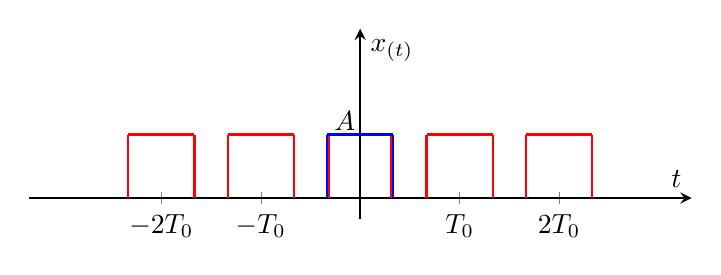
\begin{tikzpicture}
                            \begin{axis}[
                                xlabel=$t$,
                                ylabel=$x_{(t)}$,
                                xmin=-10,
                                xmax=10,
                                ymin=-0.5,
                                ymax=4,
                                ytick = {1.5},
                                xtick={-6,-3,0,3,6},
                                xticklabels={$-2T_0$,$-T_0$, $0$,$T_0$,$2T_0$},
                                yticklabels = {$A$},
                                yticklabel style = {yshift=5pt,xshift=4pt}, 
                                axis lines=middle,
                                thick,
                                domain=-5:5,
                                samples=100,
                                width=10cm,
                                height=4cm
                            ]
                            %Periodico
                            %2T0
                            \addplot [const plot, red, thick] coordinates{(-5,1.5)(-7,1.5)};
                            \addplot [const plot, red, thick] coordinates{(-5,0)(-5,1.5)};
                            \addplot [const plot, red, thick] coordinates{(-7,0)(-7,1.5)};
                            
                            \addplot [const plot, red, thick] coordinates{(5,1.5)(7,1.5)};
                            \addplot [const plot, red, thick] coordinates{(5,0)(5,1.5)};
                            \addplot [const plot, red, thick] coordinates{(7,0)(7,1.5)};

                            \addplot [const plot, red, thick] coordinates{(-2,1.5)(-4,1.5)};
                            \addplot [const plot, red, thick] coordinates{(-2,0)(-2,1.5)};
                            \addplot [const plot, red, thick] coordinates{(-4,0)(-4,1.5)};
                            
                            %T0
                            \addplot [const plot, red, thick] coordinates{(2,1.5)(4,1.5)};
                            \addplot [const plot, red, thick] coordinates{(2,0)(2,1.5)};
                            \addplot [const plot, red, thick] coordinates{(4,0)(4,1.5)};
                        
                            \addplot [const plot, red, thick] coordinates{(-0.94,1.485)(0.94,1.48)};
                            \addplot [const plot, red, thick] coordinates{(-0.94,0)(-0.94,1.48)};
                            \addplot [const plot, red, thick] coordinates{(0.94,0)(0.94,1.48)};
                        
                            %Aperiodico
                            \addplot [const plot, blue, thick] coordinates{(-1,1.5)(1,1.5)};
                            \addplot [const plot, blue, thick] coordinates{(-1,0)(-1,1.5)};
                            \addplot [const plot, blue, thick] coordinates{(1,0)(1,1.5)};
                        
                            
                            \end{axis}
                        \end{tikzpicture}
                        \caption{Segnale {\color{blue}aperiodico}, Segnale {\color{red}periodico}}
                        \label{fig:Segnale aperiodico periodico}
                    \end{figure}
                    \[
                        \begin{cases}
                            x_{(t)} \overset{TCF}{\rightleftharpoons} X_{(f)} \nonumber \\
                            y_{(t)} \overset{TSF}{\rightleftharpoons}\overunderset{+\infty}{k = -\infty}{\sum}  Y_{k} e^{j2\pi kf_0t}\nonumber
                        \end{cases}  
                        \text{Che relazione intercorre tra }Y_k\ e\ X_{(f)}
                    \]
                    \begin{align}
                        Y_k &= \frac{1}{T_0} \int_{-\frac{T_0}{2}}^{\frac{T_0}{2}} y_{(t)} e^{j2\pi kf_0t} dt =\frac{1}{T_0} \int_{-\frac{T_0}{2}}^{\frac{T_0}{2}} \overunderset{+\infty}{n = -\infty}{\sum}x_{(t-nT_0)} e^{j2\pi kf_0t} dt \nonumber \\
                                &= \frac{1}{T_0} \overunderset{+\infty}{n = -\infty}{\sum} \int_{-\frac{T_0}{2}}^{\frac{T_0}{2}} x_{(t-nT_0)} e^{j2\pi kf_0t} dt \overset{t^\prime = t-nT_0}{=} \frac{1}{T_0} \overunderset{+\infty}{n = -\infty}{\sum} \int_{-\frac{T_0}{2}-nT_0}^{\frac{T_0}{2}-nT_0} x_{(t^\prime)} e^{j2\pi kf_0(t^\prime+nT_0)} dt^\prime  \nonumber \\
                                &= \frac{1}{T_0} \overunderset{+\infty}{n = -\infty}{\sum} \int_{-\frac{T_0}{2}-nT_0}^{\frac{T_0}{2}-nT_0} x_{(t^\prime)} e^{j2\pi kf_0t^\prime} \underset{\substack{\downarrow \forall nk=1 \\\text{é la fase di un numero sempre intero nk}}\in\mathbb{N}}{e^{j2\pi nkf_0T_0}} dt^\prime\nonumber \\
                                &= \frac{1}{T_0} \overunderset{+\infty}{n = -\infty}{\sum} \int_{-\frac{T_0}{2}-nT_0}^{\frac{T_0}{2}-nT_0} x_{(t^\prime)} e^{j2\pi kf_0t^\prime}dt^\prime \rightarrow \text{$TCF$ con intervalli disgiunti e adiacenti in $kf_0$}\nonumber 
                    \end{align}
                    \begin{figure}[H]
                        \centering
                        \begin{tikzpicture}
                            \begin{axis}[
                                domain=-5:5,
                                samples=200,
                                axis lines=middle,
                                xlabel=$t$,
                                ylabel=$x_{(t)}$,
                                ymin=-0.3,
                                ymax=5,
                                xtick={-4.5,-3.5,-2.5,-1.5,-0.5,0,0.5,1.5,2.5,3.5,4.5},
                                xticklabels={$-5T_0$,$-4T_0$,$-3T_0$,$-2T_0$,$-T_0$,$0$,$T_0$,$2T_0$,$3T_0$,$4T_0$,$5T_0$},
                                ytick={},
                                width=12cm,
                                height=5cm
                            ]
                            %x(t)
                            \addplot [name path = A,const plot,black, thin] coordinates{(-5,0)(-4,0)};
                            \addplot [name path = B,domain = -5:-4,ultra thick,blue, samples = 400] {(1/5*sin(deg(x))+2)*((x/20)+1)};
                            
                            \addplot [name path = C,const plot,black, thin] coordinates{(-4,0)(-3,0)};
                            \addplot [name path = D,domain = -4:-3,ultra thick,blue, samples = 400] {(1/5*sin(deg(x))+2)*((x/20)+1)};
                            
                            \addplot [name path = E,const plot,black, thin] coordinates{(-3,0)(-2,0)};
                            \addplot [name path = F,domain = -3:-2,ultra thick,blue, samples = 400] {(1/5*sin(deg(x))+2)*((x/20)+1)};
                            
                            \addplot [name path = G,const plot,black, thin] coordinates{(-2,0)(-1,0)};
                            \addplot [name path = H,domain = -2:-1,ultra thick,blue, samples = 400] {(1/5*sin(deg(x))+2)*((x/20)+1)};
                            
                            \addplot [name path = I,const plot,black, thin] coordinates{(-1,0)(0,0)};
                            \addplot [name path = L,domain = -1:0,ultra thick,blue, samples = 400] {(1/5*sin(deg(x))+2)*((x/20)+1)};
                            
                            \addplot [name path = M,const plot,black, thin] coordinates{(0,0)(1,0)};
                            \addplot [name path = N,domain = 0:1,ultra thick,blue, samples = 400] {(1/5*sin(deg(x))+2)*((x/20)+1)};
                            
                            \addplot [name path = O,const plot,black, thin] coordinates{(1,0)(2,0)};
                            \addplot [name path = P,domain = 1:2,ultra thick,blue, samples = 400] {(1/5*sin(deg(x))+2)*((x/20)+1)};
                            
                            \addplot [name path = Q,const plot,black, thin] coordinates{(2,0)(3,0)};
                            \addplot [name path = R,domain = 2:3,ultra thick,blue, samples = 400] {(1/5*sin(deg(x))+2)*((x/20)+1)};
                            
                            \addplot [name path = S,const plot,black, thin] coordinates{(3,0)(4,0)};
                            \addplot [name path = T,domain = 3:4,ultra thick,blue, samples = 400] {(1/5*sin(deg(x))+2)*((x/20)+1)};
                            
                            \addplot [name path = U,const plot,black, thin] coordinates{(4,0)(5,0)};
                            \addplot [name path = V,domain = 4:5,ultra thick,blue, samples = 400] {(1/5*sin(deg(x))+2)*((x/20)+1)};
                            
                            \addplot [thin,black, samples = 400,black,thin] {(1/5*sin(deg(x))+2)*((x/20)+1)};
                            %Colors
                            \addplot[green,opacity = 0.3] fill between[of=A and B];
                            \addplot[blue,opacity = 0.3] fill between[of=C and D];
                            \addplot[red,opacity = 0.3] fill between[of=E and F];
                            \addplot[yellow,opacity = 0.3] fill between[of=G and H];
                            \addplot[purple,opacity = 0.3] fill between[of=I and L];
                            \addplot[black,opacity = 0.3] fill between[of=M and N];
                            \addplot[green,opacity = 0.3] fill between[of=O and P];
                            \addplot[yellow,opacity = 0.3] fill between[of=Q and R];
                            \addplot[red,opacity = 0.3] fill between[of=S and T];
                            \addplot[blue,opacity = 0.3] fill between[of=U and V];
                            \end{axis}
                        \end{tikzpicture}
                        \caption{Intervalli adiacenti e disgiunti}
                        \label{fig:Intervalli adiacenti}
                    \end{figure}
                    \[
                        Y_k = \frac{1}{T_0}\int_{-\infty}^{\infty} x_{(t^\prime)} e^{j2\pi kf_0t^\prime}dt^\prime \Rightarrow Y_k = \frac{1}{T_0} X_{(kf_0)}
                    \]
                    Sono campionamenti di $X_{(f)}$ a $kf_0$.\\
                
                \subsubsection{$I^a$ formula di Poisson}
                    \[
                        y_{(t)} \overset{TSF}{\rightleftharpoons}\overunderset{+\infty}{k = -\infty}{\sum} \frac{1}{T_0} X_{(kf_0)} e^{j2\pi kf_0t}    
                    \]
                    Evidenzia che:
                    \begin{center}
                        \emph{Periodicizzazione nel tempo} $\rightleftharpoons$ \emph{Campionamento nella frequenza}
                    \end{center}
                    \begin{figure}[H]
                        \centering
                        \begin{tikzpicture}
                            \begin{axis}[
                                domain=-5:5,
                                samples=200,
                                axis lines=middle,
                                xlabel=$f$,
                                ylabel=$X_{(f)}$,
                                ymin=-1.5,
                                ymax=1.5,
                                xtick={-4,-3,-2,-1,-0,1,2,3,4},
                                xticklabels={$-4$,$-3$,$-2$,$-1$,$-0$,$1$,$2$,$3$,$4$},
                                ytick={1},
                                yticklabels={$1$},
                                width=10cm,
                                height=6cm
                            ]
                            \addplot [red,dotted, samples = 300] {sin(deg(x*pi))/(x*pi)};
                            \addplot+ [blue,ycomb ,thin, samples at = {-1.2,-1,-0.8,-0.6,-0.4,-0.2,0,0.2,0.4,0.6,0.8,1,1.2}] {sin(deg(x*pi))/(x*pi)};
                            \end{axis}
                        \end{tikzpicture}
                        \caption{Grafico del campionamento}
                        \label{fig:campionamento in frequenza}
                    \end{figure}
                    
                    Esempio:\\
                    $y_{(t)} = |\cos(2\pi f_0t)| \hspace{.2cm} X_k = ?$
                    
                    \begin{figure}[H]
                        \centering
                        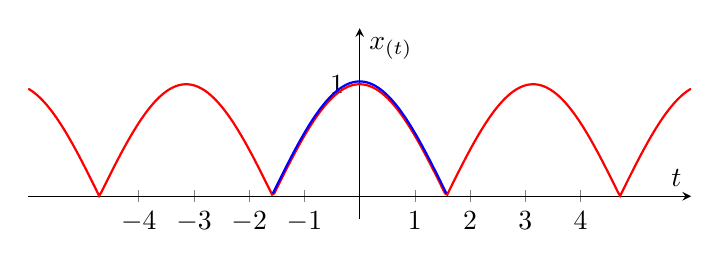
\begin{tikzpicture}
                            \begin{axis}[
                                domain=-6:6,
                                samples=200,
                                axis lines=middle,
                                xlabel=$t$,
                                ylabel=$x_{(t)}$,
                                ymin=-0.2,
                                ymax=1.5,
                                xtick={-4,-3,-2,-1,-0,1,2,3,4},
                                xticklabels={$-4$,$-3$,$-2$,$-1$,$-0$,$1$,$2$,$3$,$4$},
                                ytick={1},
                                yticklabels={$1$},
                                width=10cm,
                                height=4cm
                            ]
                            \addplot [red,thick,samples = 300] {abs(cos(deg(x)))};
                            \addplot [domain = -pi/2:pi/2,blue,thick,samples = 300] {abs(cos(deg(x))+0.025)};
                            \end{axis}
                        \end{tikzpicture}
                        \caption{$|\cos(2\pi f_0t)|$}
                        \label{fig:cos 2pif_0t}
                    \end{figure}
                    ${\color{red}y_{(t)}} = |\cos(2\pi f_0t)|$ non é altro che il segnale aperiodico ${\color{blue}x_{(t)}} = \cos(2\pi f_0t) \dotproduct rect\left(\frac{t}{\frac{T_0}{2}}\right)$ con periodo $\frac{T_0}{2}$:
                    \[
                        \begin{cases}
                            Y_k = \frac{2}{T_0} X_{(kf_0)} = \frac{2}{T_0} X_{(k\frac{2}{T_0})}   \nonumber \\
                            X_{(f)} = \frac{T_0}{2}sinc(f\frac{T_0}{2}) \otimes \left(\frac{\delta_{(f-f_0)}}{2} + \frac{\delta_{(f-f_0)}}{2}\right)\nonumber
                        \end{cases}
                    \]
                    Per il calcolo di $X_{(f)}$ si applica il Th della Modulazione con $cos$ \ref{Modulazione con coseno} e la propietá campionatrice della Delta di Dirac rispetto alla convoluzione \ref{PD3}.
                    \[
                        X_{(f)} = \frac{T_0}{4}sinc\left((f-f_0)\frac{T_0}{2}\right) + \frac{T_0}{4}sinc\left((f+f_0)\frac{T_0}{2}\right)
                    \]
                    \[
                        Y_k = \frac{2}{T_0}\frac{T_0}{4}sinc\left((\frac{2k}{T_0}-f_0)\frac{T_0}{2}\right) +\frac{2}{T_0} \frac{T_0}{4}sinc\left((\frac{2k}{T_0}+f_0)\frac{T_0}{2}\right)
                    \]
                \subsubsection{Teorema dell'integrazione completo}\label{Teorema integrazione completo}\index{Teorema dell'integrazione completo}
                    $Ip:\begin{cases}
                        x_{(t)} \overunderset{TCF}{ATCF}{\leftrightharpoons} X_{(f)}\\
                        y_{(t)} = \int_{-\infty}^{t} x_{(\alpha)} d\alpha
                    \end{cases}$\\
                    $Th: Y_{(f)} =\frac{X_{(0)}}{2}\delta_{(f)} +\frac{X_{(f)}}{j2\pi f}$ \\
                    
                    Prende la nominazione di completo perché risolve il problema di mantenere l'uguaglianza $j2\pi fY_{(f)} = X_{(f)}$
                    
                    Per la dimostrazione ci serve definire prima:
                    \begin{itemize}
                        \item{
                            $TCF$ di $\frac{1}{t}$ 
                                \begin{align}
                                    \frac{1}{t} &\overunderset{TSF}{ATSF}{\rightleftharpoons}  sgn(f) \nonumber \\
                                    \text{Per la }&\text{Dualitá \ref{Dualita}}\nonumber \\
                                    sgn(t) &\overunderset{TSF}{ATSF}{\rightleftharpoons} \frac{1}{j\pi f} \nonumber
                                \end{align}
                        }
                        \item{
                            $TCF$ del gradino $u_{(t)}$
                            \[
                              u_{(t)} = \int_{-\infty}^{\infty} \delta_{(\alpha)} d\alpha \hspace{1cm}   u_{(t)} \rightleftharpoons U_{(f)}
                            \] 
                            Non posso applicare il Th dell'integrazione \ref{Integrazione}$
                            \begin{cases}
                                y_{(+\infty)} = 1\nonumber \\    
                                \int_{-\infty}^{\infty} u_{(t)} dt  = 1\nonumber \\   
                                X_{(f)} = 1 \nonumber    
                            \end{cases}$
                            la terza ipotesi non é mai verificata. Scriviamo la funzione gradino in modo diverso:
                            \[
                                u_{(t)} = \frac{1}{2}+\frac{1}{2}sgn(t)
                            \] 
                            \begin{figure}[H]
                                \centering
                                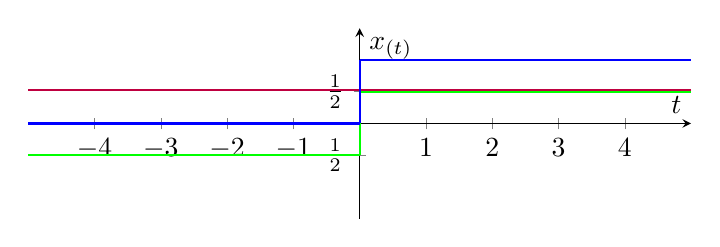
\begin{tikzpicture}
                                    \begin{axis}[
                                        domain=-5:5,
                                        samples=200,
                                        axis lines=middle,
                                        xlabel=$t$,
                                        ylabel=$x_{(t)}$,
                                        ymin=-1.5,
                                        ymax=1.5,
                                        xtick={-4,-3,-2,-1,-0,1,2,3,4},
                                        xticklabels={$-4$,$-3$,$-2$,$-1$,$-0$,$1$,$2$,$3$,$4$},
                                        ytick={-0.5,0.5},
                                        yticklabels={$-\frac{1}{2}$,$\frac{1}{2}$},
                                        width=10cm,
                                        height=4cm
                                    ]
                                    %const
                                    \addplot [const plot,thick,purple] coordinates{(-5,0.525)(5,0.525)};

                                    %sgn
                                    \addplot [const plot,thick,green] coordinates{(0,0.5)(5,0.5)};
                                    \addplot [const plot,thick,green] coordinates{(0,-0.5)(-5,-0.5)};
                                    \addplot [const plot,thick,green] coordinates{(0,-0.5)(0,0.5)};

                                    %u(t)
                                    \addplot [const plot,thick,blue] coordinates{(0,0)(-5,0)};
                                    \addplot [const plot,thick,blue] coordinates{(0,0)(0,1)};
                                    \addplot [const plot,thick,blue] coordinates{(0,1)(5,1)};
                                    \end{axis}
                                \end{tikzpicture}
                                \caption{${\color{blue}u_{(t)}} = {\color{purple}\frac{1}{2}}+{\color{green}\frac{1}{2}sgn(t)}$}
                                \label{fig:gradino alternativo}
                            \end{figure}
                            \[
                                U_{(f)} = TCF[u_{(t)}] = \frac{1}{2}\delta_{(f)}+\frac{1}{2j\pi f}
                            \]
                            \[
                                \frac{1}{2}+\frac{1}{2}sgn(t) \overunderset{TSF}{ATSF}{\rightleftharpoons} \frac{1}{2}\delta_{(f)}+\frac{1}{2j\pi f} 
                            \]
                        }
                    \end{itemize}                    

                    
                    Dimostrazione Th. Integrazione completo:\\
                        \[
                            y_{(t)} = \int_{-\infty}^{t} x_{(\alpha)} d\alpha =\int_{-\infty}^{\infty} x_{(\alpha)} u_{(t-\alpha)} d\alpha
                        \]
                        \begin{figure}[H]
                            \centering
                            \begin{tikzpicture}
                                \begin{axis}[
                                    domain=-5:5,
                                    samples=200,
                                    axis lines=middle,
                                    xlabel=$t$,
                                    ylabel=$x_{(t)}$,
                                    ymin=-0.3,
                                    ymax=5,
                                    xtick={-4,-3,-2,-1,-0,1,2,3,4},
                                    xticklabels={$-4$,$-3$,$-2$,$-1$,$-0$,$1$,$2$,$3$,$4$},
                                    ytick={},
                                    width=12cm,
                                    height=5cm
                                ]
                                %x(t)
                                \addplot [name path = A,const plot,black, thin] coordinates{(-5,0)(2,0)};
                                \addplot [name path = B,domain = -5:2,ultra thick,blue, samples = 400] {(1/5*sin(deg(x))+2)*((x/20)+1)};
                                \addplot [thin,black, samples = 400,black,thin] {(1/5*sin(deg(x))+2)*((x/20)+1)};
                                %u(t)
                                \addplot [const plot,red] coordinates{(-5,1)(2,1)};
                                \addplot [const plot,red] coordinates{(2,0)(5,0)};
                                \addplot [const plot,red] coordinates{(2,0)(2,1)};

                                \addplot[green,opacity = 0.3] fill between[of=A and B];
                                \end{axis}
                            \end{tikzpicture}
                            \caption{${\color{green}y_{(t)}} = \int_{-\infty}^{\infty} {\color{black}x_{(\alpha)}} {\color{red}u_{(t-\alpha)}} d\alpha, {\color{blue}x_{(\alpha)}u_{(t-\alpha)}} $}
                            \label{fig:gradino che limite la funzione}
                        \end{figure}
                        Utilizziamo il gradino per cambiare gli estremi dell'integrale e mantenere il valore di $x_{(t)}$ dopo $t$ a $0$. Ci siamo ricondotti all'integrale di convoluzione \ref{Convoluzione} nel tempo,
                        quindi nella frequenza diventa un prodotto:
                        \[
                            Y_{(f)} =X_{(f)} U_{(f)} = \frac{X_{(f)}}{2}\delta_{(f)} +\frac{X_{(f)}}{j2\pi f} =\frac{X_{(0)}}{2}\delta_{(f)} +\frac{X_{(f)}}{j2\pi f}    
                        \]
                        Se $X_{(0)}$ fosse $0$ avrei il classico Th. dell'integrazione.
                        DOMANDA: ma quindi nella propietá campionatrice in frequenza rimane la delta????